% Tento soubor nahraďte vlastním souborem s obsahem práce.
%=========================================================================
% Autoři: Michal Bidlo, Bohuslav Křena, Jaroslav Dytrych, Petr Veigend a Adam Herout 2019

% Pro kompilaci po částech (viz projekt.tex), nutno odkomentovat a upravit
%\documentclass[../projekt.tex]{subfiles}
%\begin{document}

\listofdotazy
\listoftodos

\chapter{Úvod}\label{kap_uvod}
Jednou z~oblastí, kterou se zabývá teoretická informatika, je teorie formálních jazyků.
Tato oblast využívá jednoduchých konceptů, jako jsou množiny, relace, symboly a~řetězce, k~popisu konceptů složitějších\,--\,například programovacích jazyků.
Programovací jazyky jsou kompromisem mezi přirozenými a~strojovými jazyky, nicméně od posloupnosti nul a~jedniček, kterým počítač rozumí, mají daleko.
Jsou ale navrhnuty tak, aby do nul a~jedniček byly algoritmicky přeložitelné a~zároveň poskytovaly takovou abstakci, která je člověku, respektive programátorovi, srozumitelná.  

Mezi kroky překladu se mimo jiné řadí lexikální, syntaktická a~sémantická analýza, generování mezikódu a~generování cílového kódu.
Syntaktická analýza hraje v~procesu překladu klíčovou roli, ne-li nejdůležitější\,--\,moderní překladače dokonce často používají paradigma \emph{syntaxí řízeného překladu}.
Je to proces, který ověřuje správnost posloupnosti jednotlivých symbolů řetězce, který má syntaktický analyzátor na vstupu.
Přesněji řečeno zkontroluje, zda vstupní řetězec mohl být vygenerován modelem, který daný programovací jazyk popisuje.

Nejčastěji používaný model pro popis jazyka je gramatika.
Gramatiky jsou čtyř typů a~vytváří hierarchii generativní síly podle typu pravidel, které jsou v~nich použity.
Tuto skutečnost popsal americký filozof a~lingvista Noam Chomsky v~roce 1956.
Tato práce se zabývá pouze jedním typem gramatik, a~to jsou gramatiky bezkontextové, také nazývané gramatiky typu 2.
Přesněji LL~gramatikami, které mají menší generativní sílu než bezkontextové, nicméně jazyky generované těmito modely mohou být přijímány relativně jednoduchými a~hlavně deterministickými konstrukcemi, jako je například deterministický zásobníkový automat.
Díky tomu je tento typ gramatik v~praxi velmi rozšířený pro budování syntaktických analyzátorů.
Dokonce existuje několik nástrojů, které syntaktické analyzátory automaticky generují z~LL gramatik napsaných ve speciální syntaxi.

Velký trend teoretické informatiky na přelomu 20.~a~21.~století byl výzkum gramatických systémů.
Bylo v~zájmu příjít na způsob popsání jazyka několika gramatikami, jejichž spolupráce vyústila ve větší generativní sílu systému oproti samostatným gramatikám stejného typu.
Nakonec se uchytily především kooperující distribuované (CD) a~paralelní komunikující (PC) gramatické systémy.

Tato práce se zabývá upravením principu syntaktické analýzy jazyka popsaného LL gramatikou pro CD gramatický systém.
Cílem je navrhnout CD gramatický systém popisující ekvivalentní jazyk jako LL gramatika a~následně implementovat syntaktický analyzátor pomocí deterministického zásobníkového automatu, který tento jazyk přijímá.
Pro návrh analyzátoru budou použity množiny $Empty$, $First$, $Follow$ a~$Predict$, které se standardně využívají k~návrhu LL tabulky, která je nedílnou součástí syntaktických analyzátorů.
Pro výrazy bude využita precedenční analýza.  

V~Kapitole~\ref{kap_teorie} jsou popsány základní pojmy a~principy teorie formálních jazyků, které jsou prerekvizitou k~pochopení této práce.
Kapitola~\ref{kap_GS} zavádí nové teoretické koncepty v~podobě gramatických systémů jako rozšíření klasických gramatik.
Principy syntaktické analýzy jsou popsány v~Kapitole~\ref{kap_teorie_sa}, která zároveň uvádí algoritmy pro sestavení potřebných množin a~tabulek, se kterými syntaktický analyzátor pracuje.
Vlastní principy implementace systému na abstraktní úrovni jsou popsány v~Kapitole \ref{kap_implementace}.
Zároveň se zmiňuje o~implementačním jazyce, adresářové struktuře, sestavovacím systému a~podobně.
Poslední kapitola pak pojednává o~testování implementovaného systému.

\chapter{Základy teorie formálních jazyků}\label{kap_teorie}
Základní přehled matematických znalostí potřebných k~pochopení této kapitoly (a~tím i~celé této práce) je popsán například v~\cite{meduna_zemek_2014}.

\section{Abeceda, řetězec a jazyk}\label{kap_abec_ret_jazyk}
Definice v~této kapitole založeny na definicích z~\cite{hopcroft2006introduction, handbook1-zaklady, TIN-opora}.

\subsection*{Abecedy, řetězce a operace s nimi}

\begin{definition}
    \emph{Abeceda} je neprázdná množina prvků, které se nazývají \emph{symboly} nebo \emph{písmena}.
\end{definition}

\begin{convention}
    Abeceda se označuje velkými písmeny řecké abecedy; v~této práci bude použito výhradně písmeno $\Sigma$ (\emph{sigma}).
\end{convention}

\begin{definition}
    Nechť $\Sigma$ je abeceda. \\
    \emph{Slovo} nebo \emph{řetězec} nad abecedou $\Sigma$ je konečná posloupnost symbolů z~$\Sigma$, symbol se může v~řetězci několikrát opakovat.
    Formálně se dá zapsat jako posloupnost
    \begin{equation*}
        x = (a_1, a_2, \ldots, a_n),\; n \geq 0,\; a_i \in \Sigma \text{ pro všechna } i \in \{1, \ldots ,n\}\; \cite{harag2023}.
    \end{equation*}
    Speciálním případem je \emph{prázdný řetězec} pro $n = 0$, označuje se písmenem $\varepsilon$.
\end{definition}

\begin{convention}
    Při zápisu řetězců je jednodušší vynechat závorky a~oddělovače symbolů.
    Proto zápis $(a_1, a_2, \ldots, a_n)$ je ekvivalentní se zápisem $a_1a_2\ldots a_n$ \cite{meduna2014formal}.
    
    Řetězce v~této práci budou označovány malými písmeny abecedy stejně jako symboly.
    Pro řetězce budou používána písmena z~konce abecedy ($w$, $x$, $y$, $z\,$ a~podobně), pro symboly písmena ze začátku abecedy ($a$, $b$, $c\,$ a~podobně).
\end{convention}

\begin{definition}
    Nechť $\Sigma$ je abeceda $x = a_1a_2\ldots a_n$ je řetězec nad $\Sigma$.\\
    \emph{Délka řetězce x} je počet pozic se symboly z~abecedy $\Sigma$ v~řetězci, značí se $|x|$.
    Dále $alph(x)$ označuje množinu symbolů, které se v~řetězci $x$ vyskytují.
\end{definition}

\begin{definition}
    Nechť $\Sigma$ je abeceda $x = a_1a_2\ldots a_n$ je řetězec nad $\Sigma$.\\
    \emph{Reverzace} řetězce $x$, $reversal(x)$ nebo také $x^R$ je
    \begin{equation*}
        x^R = x_nx_{n-1}\ldots x_1x_0.
    \end{equation*} 
    Prázdný řetězec zřejmě bude stejný, jako jeho reverzace.
    \begin{equation*}
        \varepsilon^R = \varepsilon
    \end{equation*}
\end{definition}

\begin{definition}
    Nechť $\Sigma$ je abeceda a~$w$ je řetězec nad $\Sigma$.\\
    Řetězec $z$ je \emph{podřetězec} řetězce $w$, jestliže existují řetězce $x$ a~$y$ takové, že
    \begin{equation*}
        w = xzy.
    \end{equation*}
    Řetězec $x_1$ je prefixem (předponou) řetězce $w$, jestliže existuje řetězec $y_1$ takový, že
    \begin{equation*}
        w = x_1y_1.
    \end{equation*}
    Řetězec $x_2$ je sufixem (příponou) řetězce $w$, jestliže existuje řetězec $y_2$ takový, že
    \begin{equation*}
        w = y_2x_2.
    \end{equation*}
    Je-li $y_1 \neq \varepsilon$, pak $x_1$ je \emph{vlastní prefix} řetězce $w$; je-li $y_2 \neq \varepsilon$, pak $x_2$ je \emph{vlastní sufix} řetězce $w$.
\end{definition}

\begin{definition}
    Nechť $\Sigma$ je abeceda.\\
    Množina všech řetězců abecedy $\Sigma$ určité délky $k$ je $\Sigma^k$.
    $\Sigma^0 = \{\varepsilon\}$ pro libovolnou abecedu.
\end{definition}

\begin{example}
    Nechť $\Sigma = \{0, 1\}$ je abeceda.\\
    Všechny řetězce délky 2 jsou $00,\; 01,\; 10,\; 11$.
    Zřejmě tedy $\Sigma^2 = \{00,\; 01,\; 10,\; 11\}$.
\end{example}

\begin{definition}
    Nechť $\Sigma$ je abeceda.\\
    Množina všech řetězců nad abecedou $\Sigma$ je
    \begin{equation*}
        \Sigma^* = \Sigma^0 \cup \Sigma^1 \cup \Sigma^2 \cup \cdots
    \end{equation*}
    a~množina všech \emph{neprázdných} řetězců nad abecedou $\Sigma$ je
    \begin{equation*}
        \Sigma^+ = \Sigma^1 \cup \Sigma^2 \cup \Sigma^3 \cup \cdots \text{ nebo } \Sigma^+ = \Sigma^* \setminus \{\varepsilon\}.
    \end{equation*}
\end{definition}

\begin{definition}
    Nechť $\Sigma$ je abeceda a~$x = a_1a_2\ldots a_i$ a~$y = b_1b_2\ldots b_j$ jsou řetězce nad $\Sigma$.\\
    \emph{Konkatenace řetězců}, symbolicky zapsána $xy$, je
    \begin{equation*}
        xy = a_1a_2\ldots a_ib_1b_2\ldots b_j.
    \end{equation*}
    Jinými slovy, vznikne nový řetězec spojením $x$ a~$y$ hned za sebe.
    Konkatenace řetězce s~prázdným řetězcem v~libovolném pořadí nemění původní řetězec.
    \begin{equation*}
        \varepsilon x = x\varepsilon = x
    \end{equation*}
\end{definition}

\begin{example}
    Nechť $\Sigma = \{0, 1\}$ je abeceda, $x = 011$, $y = 1101$ řetězce nad $\Sigma$.\\
    Konkatenace řetězců $xy = 0111101$ a~$yx = 1101011$.
\end{example}

\subsection*{Jazyky a operace s nimi}
\begin{definition}
    Nechť $\Sigma$ je abeceda. \\
    Jazyk $L$ nad abecedou $\Sigma$ je konečná či nekonečná množina řetězců nad $\Sigma$, nebo také $L \subseteq \Sigma^*$.
    Řetězce jazyka se nazývají \emph{věty} nebo \emph{slova}.

    Množiny $\emptyset$ a~$\{\varepsilon\}$ jsou jazyky nad libovolnou abecedou $\Sigma$, nicméně $\emptyset \neq \{\varepsilon\}$. $\emptyset$ je jazyk, který neobsahuje žádné řetězce, zatímco $\{\varepsilon\}$ obsahuje právě jeden řetězec, a~to prázdný.
\end{definition}

\begin{definition}
    Nechť $L_1$ a~$L_2$ jsou jazyky nad $\Sigma$.\\
    Typické množinové operace mohou jsou použitelné i pro jazyky:
    \begin{itemize}
        \item sjednocení jazyků je definováno jako 
        \begin{equation*}
            L_1 \cup L_2 = \{x : x \in L_1 \vee x \in L_2\},
        \end{equation*}
        \item průnik jazyků je definován obdobně jako
        \begin{equation*}
            L_1 \cap L_2 = \{x : x \in L_1 \wedge x \in L_2\},
        \end{equation*}
        \item rozdíl jazyků je
        \begin{equation*}
            L_1 \setminus L_2 = \{x : x \in L_1 \wedge x \notin L_2\}.
        \end{equation*} 
    \end{itemize}
    Pro jazyky existuje speciální operace \emph{konkatenace}, která vychází z~konkatenace řetězců:
    \begin{equation*}
        L_1L_2 = \{xy : x \in L_1 \wedge y \in L_2\}.   
    \end{equation*} 
\end{definition}

\begin{definition}
    Nechť $\Sigma$ je abeceda a~$L$ jazyk nad $\Sigma$.\\
    \emph{Reverzace} jazyka, $reversal(L)$ nebo $L^R$ je
    \begin{equation*}
        L^R = \{x^R : x \in L\},
    \end{equation*}
    \emph{mocnina} jazyka $L^i$ je definována jako
    \begin{alignat*}{-1}
        \text{1)}& \quad L^0 &&= \{\varepsilon\},\\
        \text{2)}& \quad L^i &&= LL^{i-1},\; i \geq 0,
    \end{alignat*}
    \emph{iterace} jazyka je sjednocení všech mocnin jazyka:
    \begin{equation*}
        L^* = \bigcup_{n \geq 0} L^n,
    \end{equation*}
    \emph{pozitivní iterací} rozumíme obyčejnou iteraci bez nulté mocniny:
    \begin{equation*}
        L^+ = \bigcup_{n \geq 1} L^n.
    \end{equation*}
    Z těchto definic dále vyplývá 
    \begin{align*}
        L^* &= L^+ \cup \{\varepsilon\},\\
        L^+ &= L^*L = LL^*,
    \end{align*}
    důkaz lze nalézt například v~\cite{TIN-opora}.
\end{definition}

\section{Gramatika}

Informace pro tuto kapitolu byly převzaty z~\cite{TIN-opora}.

V~Kapitole \ref{kap_abec_ret_jazyk} byly ukázány obecné a~pouze základní principy jazyků.
S~triviálními způsoby reprezentace jazyka, tedy například výčtem všech vět, si nevystačíme už jen díky tomu, že jazyky často bývají nekonečné.
Gramatiky jsou jedním ze způsobů, a~to velmi elegantním, jak jazyky reprezentovat.

Používají dva typy symbolů\,--\,\emph{nonterminální} symboly a~\emph{terminální} symboly.
Nonterminální symboly slouží k~popisu syntaktických celků jazyka a~terminální symboly se shodují se symboly ze vstupní abecedy.

\begin{convention}
    Pro nonterminální symboly bude dále v~práci používáno zkrácené označení \emph{neterminály} a~pro terminální symboly pojem \emph{terminály}.
\end{convention}

\begin{convention}\label{conv_oznaceni_symbolu}
    V~kontextu práce s~gramatikami bude nadále používáno následující označení pro různé typy řetězců:
    \begin{itemize}
        \item malá písmena ze začátku abecedy ($a, b, c,\ldots)$ budou reprezentovat terminály,
        \item velká písmena ze začátku abecedy ($A, B, C,\ldots)$ budou vyhrazena pro neterminály,
        \begin{itemize}[label=$\circ$]
            \item výjimkou je symbol $S$, který je často používán pro označení \emph{startovacího symbolu},
        \end{itemize}
        \item malá písmena ze začátku řecké abecedy $(\alpha, \beta, \gamma,\ldots)$ budou označovat řetězce terminálů a~neterminálů,
        \item malá písmena z~konce abecedy ($u, v, w,\ldots$) budou pro řetězce terminálů.
    \end{itemize}
\end{convention}

Gramatika představuje generativní systém, ve kterém lze z jistého vyznačeného neterminálu generovat, aplikací \emph{přepisovacích pravidel}, řetězce tvořené neterminálními a~terminálními symboly, které nazýváme \emph{větnými formami}. 
Větné formy, které jsou tvořeny pouze terminálními symboly, reprezentují věty gramatikou definovaného jazyka.
Pokud gramatika negeneruje žádnou větu, pak reprezentuje prázdný jazyk.

Přepisovací pravidla jsou jádrem gramatik.
Jejich využití spočívá v~neustálém přepisování neterminálních symbolů, dokud není vygenerován řetězec terminálů (podrobněji v~definicích \ref{def_derivacni_krok}, \ref{def_der_krok_tranz} a~\ref{def_der_krok_refl_tranz}).
Každé pravidlo je ve tvaru uspořádané dvojice $(\alpha, \beta)$ řetězců, kdy se při aplikaci tohoto pravidla podřetězec $\alpha$ nahradí řetězcem $\beta$.
Podmínkou je, aby $\alpha$ obsahoval alespoň jeden neterminál.

\begin{definition}\label{def_gramatika}
    Gramatika $G$ je čtveřice $G = (N, T, P, S)$, kde
    \begin{itemize}
        \item $N$ je konečná množina neterminálů,
        \item $S$ je konečná množina terminálů,
        \item $P$ je konečná relace $R \subseteq (N \cup T)^*N(N \cup T)^* \times (N \cup T)^*$,
        \item $S$ je počáteční (výchozí, startovací) symbol gramatiky.
    \end{itemize}
    Prvek $(\alpha, \beta) \in P$ (\emph{přepisovací pravidlo}) bývá zjednodušeně zapisováno jako $\alpha \rightarrow \beta$.
\end{definition}
V~následujícím příkladě je ukázka gramatiky v~obecném tvaru.
\begin{example}
    \begin{gather*}
        G = (\{A, S\},\; \{0, 1\},\; P,\; S) \\
        P = \{S \rightarrow 0A1,\; 0A \rightarrow 00A1, A \rightarrow \varepsilon\}
    \end{gather*}
\end{example}

\subsection*{Derivační krok}\label{kap_der_krok}
Myšlenkou derivačního kroku je přepsat aktuální řetězec na řetězec nový za použití přepisovacího pravidla $p \in P$.
\begin{definition}\label{def_derivacni_krok}
    Nechť $G = (N, T, P, S)$ je gramatika, $\lambda, \mu  \in (N \cup T)^*$ a $p = \alpha \rightarrow \beta \in P$. \\
    Mezi řetězci $\lambda$ a~$\mu$ platí binární relace $\underset{\scriptscriptstyle G}{\Rightarrow}$, nazývaná \emph{přímá derivace}, jestliže můžeme řetězce $\lambda$ a~$\mu$ vyjádřit ve tvaru
    \begin{align*}
        \lambda &= \gamma \alpha \delta \\
        \mu &= \gamma \beta \delta 
    \end{align*}
    kde $\gamma$ a~$\delta$ jsou libovolné řetězce z~$(N \cup T)^*$. 
    Říkáme také, že gramatika $G$ provádí \emph{derivační krok} z~$\gamma \alpha \delta$ do $\gamma \beta \delta$, respektive z~$\lambda$ do $\mu$.
\end{definition}
To znamená, že pokud lze přepsat řetězec $\lambda = \gamma \alpha \delta$ na řetězec $\mu = \gamma \beta \delta$ za použití pravidla $\alpha \rightarrow \beta$, potom mezi řetězci $\alpha$ a~$\beta$ je relace přímé derivace, zapsáno $\alpha \Rightarrow \beta$.

\begin{figure}[ht]\label{fig_der_krok}
    \centering
    \vspace*{0.5em}
    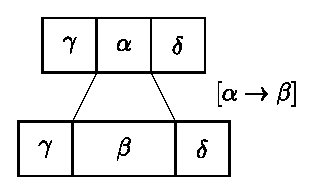
\includegraphics{obrazky-figures/derivacni_krok_bkg.eps}
    \caption{Ilustrace derivačního kroku za použití pravidla $\alpha \rightarrow \beta$.}
\end{figure}

\subsection*{Sekvence derivačních kroků}\label{kap_sekvence_der_kroku}
\begin{definition}\label{def_der_krok_tranz}
    Nechť $G = (N, T, P, S)$ je gramatika a~$\lambda, \mu \in (N \cup T)^*$. \\
    Mezi řetězci $\lambda$ a $\mu$ platí relace $\Rightarrow^+$ nazývaná \emph{derivace}, jestliže existuje posloupnost přímých derivací $\chi_{i-1} \Rightarrow \chi_i, i \in \{1, \ldots, n\}, n \geq 1$ taková, že platí
    \begin{center}
        $\lambda = \chi_0 \Rightarrow \chi_1 \Rightarrow \ldots \Rightarrow \chi_{n-1} \Rightarrow \chi_n = \mu$.
    \end{center}
    Tato posloupnost se nazývá \emph{derivace délky n}.
    Platí-li $\lambda \Rightarrow \mu$, pak řetězec $\mu$ lze \emph{generovat} z~řetězce $\lambda$, nebo také $\mu$ je \emph{derivovatelný} z~$\lambda$ v~gramatice $G$.
    Relace $\Rightarrow^+$ je tranzitivním uzávěrem relace přímé derivace $\Rightarrow$.
    Symbolem $\Rightarrow^n$ se značí n-tá mocnina přímé derivace $\Rightarrow$.
\end{definition}
Jinými slovy, pokud řetězec $\lambda$ derivuje řetězec $\chi$ v~nenulovém počtu kroků a~zároveň $\chi$ derivuje řetězec $\mu$ v~nenulovém počtu kroků, pak je zřejmé, že $\lambda$ derivuje $\mu$ v~nenulovém počtu kroků, zapsáno $\lambda \Rightarrow^+ \mu$. 

\begin{definition}\label{def_der_krok_refl_tranz}
    Nechť $G = (N, T, P, S)$ je gramatika a~$\lambda, \mu \in (N \cup T)^*$. \\
    Jestliže v~$G$ platí pro řetězce $\lambda$ a~$\mu$ relace $x \Rightarrow^+ y$ nebo identita $\lambda = \mu$, pak $\lambda \Rightarrow^* \mu$.
    Relace~$\Rightarrow^*$ je reflexivním a~tranzitivním uzávěrem relace přímé derivace $\Rightarrow$.  
\end{definition}
Reflexivní uzávěr relace přímé derivace $\Rightarrow$ znamená, že řetězec přímo derivuje sám sebe v~nula krocích.
Také je možné říci, že se nepoužije žádné pravidlo k~přepsání řetězce na sebe sama, zapsáno $\lambda \Rightarrow^0 \lambda$.

\section{Chomského hierarchie gramatik}\label{kap_chomsky_hierarchie}
Informace k~následující kapitole převzaty z~\cite{TIN-opora}.

Gramatiky se dělí do čtyř skupin podle tvaru přepisovacích pravidel.
Označují se jako typ 0, typ 1, typ 2, typ 3, respektive neomezené gramatiky, kontextové gramatiky, bezkontextové gramatiky a~pravé lineární gramatiky.
Tyto gramatiky generují příslušné jazyky $L_i,\; i \in \{0, 1, 2, 3\},$ $i$ je příslušné s~typem gramatiky.
Platí $L_3 \subseteq L_2 \subseteq L_1 \subseteq L_0$.

\subsection*{Neomezená gramatika}
Gramatika typu 0 obsahuje pravidla v~nejobecnějším tvaru, shodným z~Definice \ref{def_gramatika}.
\begin{equation*}
    \alpha \rightarrow \beta,\; \alpha \in (N \cup T)^*N(N \cup T)^*,\; \beta \in (N \cup T)^*
\end{equation*}

\subsection*{Kontextová gramatika}
Gramatika typu 1 obsahuje pravidla ve tvaru:
\begin{equation*}
    \alpha A \beta \rightarrow \alpha \gamma \beta,\; A \in N,\; \alpha, \beta \in (N \cup T)^*,\; \gamma \in (N \cup T)^+
\end{equation*}
nebo $S \rightarrow \varepsilon$, pokud se $S$ nevyskytuje na pravé straně žádného pravidla.
\begin{example}
    Příklad kontextové gramatiky:
    \begin{align*}
        G \; &= \; (\{A, S\}, \{0, 1\}, P, S) \text{ s~pravidly }\\
        S \; &\rightarrow \; 0A \; | \; \varepsilon \\ 
        0A \; &\rightarrow \; 00A1 \\
        A \; &\rightarrow \; 1
    \end{align*}
\end{example}

Těmto gramatikám se říká \emph{kontextové}, protože neterminál $A$ může být přepsán řetězcem $\gamma$ pouze tehdy, když jeho levým kontextem je řetězec $\alpha$ a~jeho pravým kontextem řetězec $\beta$.
Tyto gramatiky nepřipouštějí, aby neterminál byl nahrazen prázdným řetězcem, tedy zakazuje pravidla ve tvaru
\begin{equation*}
    \alpha A \beta \rightarrow \alpha \beta,
\end{equation*}
kromě výše zmiňované výjimky se startovacím symbolem $S$.

\subsection*{Bezkontextová gramatika}
Práce s~gramatikami typu 2 je jedním z~jader této práce.
Definujme tedy tento typ gramatiky podrobněji než ostatní typy.
\begin{definition}\label{def_bkg}
    \emph{Bezkontextová gramatika} je čtveřice $G = (N, T, P, S)$, kde:
    \begin{itemize}
        \item $N,\; T,\; S$ jsou definovány stejně jako v~Definici \ref{def_gramatika}, 
        \item $P$ je množina přepisovacích pravidel ve tvaru $A \rightarrow \gamma $, $A \in N$ a $\gamma \in (N \cup T)^*$,
        \begin{itemize}[label=$\circ$]
            \item je tudíž podmnožinou kartézského součinu $P \subseteq  N \times (N \cup T)^*$. 
        \end{itemize}
    \end{itemize}
\end{definition}

\begin{convention}
    Pro označení bezkontextových gramatik bude v~textu dále využívána zkratka BKG.
\end{convention}

Substituci neterminálu $A$ je možné provést bez závislosti na pravém a~levém kontextu, ve kterém je neterminál $A$ uložen.
Tyto gramatiky smějí obsahovat pravidla ve tvaru $A \rightarrow \varepsilon$.

\begin{example}
    Příklad bezkontextové gramatiky:
    \begin{align*}
        G \; &= \; (\{S\}, \{0, 1\}, P, S) \text{ s~pravidlem } \\
        S \; &\rightarrow \; 0S1 \; | \; \varepsilon
    \end{align*}
\end{example}

\subsection*{Pravá lineární gramatika}
Gramatika typu 3 obsahuje pravidla ve tvaru
\begin{equation*}
    A \rightarrow xB \text { nebo } A \rightarrow x,\; A, B \in N,\; x \in T^*.
\end{equation*}
Jediný možný neterminál v~pravidlech stojí úplně vpravo, proto \emph{pravá lineární} gramatika.
Další možný název je \emph{regulární gramatika}.

\begin{example}
    Příklad pravé lineární gramatiky:
    \begin{align*}
        G \; &= \; (\{A, B\}, \{a, b, c\}, P, S) \text{ s~pravidly } \\
        A \; &\rightarrow \; aaB \; | \; ccB \\
        B \; &\rightarrow \; bB \; | \; \varepsilon
    \end{align*}
\end{example}

\section{Konečný automat}
Definice související s~konečnými automaty převzaty z~\cite{meduna2023automata}, není-li řečeno jinak.
\begin{definition}\label{def_konecny_automat}
    \emph{Konečný automat} je pětice
    \begin{equation*}
        M = (Q, \Sigma, R, s, F),
    \end{equation*}
    kde
    \begin{itemize}
        \item $Q$ je konečná množina stavů,
        \item $\Sigma$ je konečná vstupní abeceda, $Q \cap \Sigma = \emptyset$,
        \item $R$ je konečná relace, $R \subseteq Q \times (\Sigma \cup \{\varepsilon\}) \times Q$,
        \begin{itemize}[label=$\circ$]
            \item je nazývána \emph{množinou pravidel} ve tvaru $qa \rightarrow p,\; q, p \in Q,\;a \in \Sigma \cup \{\varepsilon\}$.
            Jakákoli uspořádaná trojice $(q, a, p) \in R$ je pravidlem, zapsáno $qa \rightarrow p$.
        \end{itemize}
        \item $s \in Q$ je počáteční stav automatu,
        \item $F \subseteq Q$ je konečná množina koncových stavů. 
    \end{itemize}
\end{definition}

\begin{convention}
    Pro označení konečných automatů bude dále v~textu použito zkrácené KA. 
\end{convention}

U~konečných automatů popisujeme jejich \emph{konfiguraci}\,--\,ve kterém stavu se nachází a~jaký řetězec na vstupní pásce.
\begin{definition}\label{def_konfigurace_ka}
    Nechť $M = (Q, \Sigma, R, s, F)$ je KA. Dle autorů v~\cite{TIN-opora} je konfigurace $M$ uspořádaná dvojice
    \begin{equation*}
        (q, w) \in Q \times \Sigma^*.
    \end{equation*} 
    Nechť $X_M$ značí množinu všech konfigurací $M$.
\end{definition}

Pomocí konfigurací můžeme definovat \emph{přechody} KA, které reprezentují jejich výpočetní kroky.
Výpočetní krok znamená přechod z~jedné konfigurace do druhé za přečtení symbolu ze vstupní pásky.
\begin{definition}\label{def_prechod_ka}
    Nechť $M = (Q, \Sigma, R, s, F)$ je KA.\\
    Binární relace $\vdash_{\scriptscriptstyle M}$, nazývána přechodem KA $M$, je
    \begin{equation*}
        \beta\; \vdash_{\scriptscriptstyle M}\chi,
    \end{equation*}
    kde $\beta = (q, ax),\, \chi = (p, x) \in X_M,$ a~$qa \rightarrow p \in R$.
    Je to binární relace na množině konfigurací\,--\,pokud $\beta\, \vdash_{\scriptscriptstyle M} \chi$, pak $(\beta, \chi) \in X_M \times X_M$.
    Pokud $a = \varepsilon$, není ze vstupní pásky přečten žádný symbol.
    
    Symboly $\vdash_{\scriptscriptstyle M}^n, \vdash_{\scriptscriptstyle M}^+$ a~$\vdash_{\scriptscriptstyle M}^*$ nechť značí příslušně $n$-tou mocninu pro $n \geq 0$, tranzitivní a reflexivně-tranzitivní uzávěr relace $\vdash_{\scriptscriptstyle M}$ podobně jako u~derivačního kroku gramatik v~Definici \ref{def_derivacni_krok}, čímž reprezentují \emph{sekvenci přechodů} KA $M$.
    Například pro konfigurace $\beta$ a~$\chi$ platí $\beta\; \vdash_{\scriptscriptstyle M}^+ \chi$ právě tehdy, když
    \begin{equation*}
        \beta = c_0 \vdash_{\scriptscriptstyle M} c_1 \vdash_{\scriptscriptstyle M} \ldots \vdash_{\scriptscriptstyle M} c_{n-1} \vdash_{\scriptscriptstyle M} c_{n} = \chi,
    \end{equation*}
    pokud $\beta, \chi, c_1, \ldots, c_{n-1} \in X_M,\; n \geq 1$.
\end{definition}

\begin{convention}
    Bude-li z~kontextu jasné, že se jedná o~přechod automatu~$M$, pak bude relace přechodu $\vdash$ psána bez indexu $M$.  
\end{convention}

\begin{definition}
    Nechť $M = (Q, \Sigma, R, s, F)$ je KA.\\
    Jazyk přijímaný $M$, značen $L(M)$, je
    \begin{equation*}
        L(M) = \{w \in \Sigma^*: sw\; \vdash^* f,\; f \in F\}.
    \end{equation*}
    Jsou to řetězce takové, po jejichž zpracování skončí $M$ v~koncovém stavu.
\end{definition}


\begin{definition}
    Nechť $M = (Q, \Sigma, R, s, F)$ je KA.\\
    $M$ je \emph{KA bez $\varepsilon$-přechodů}, pokud pro každé pravidlo $qa \rightarrow p \in R$ platí, že $a \neq \varepsilon$.
\end{definition}

\begin{definition}
    Nechť $M = (Q, \Sigma, R, s, F)$ je KA bez $\varepsilon$-přechodů.\\
    $M$ je \emph{deterministický KA} právě tehdy, když pro každé $q \in Q$ a~každé $a \in \Sigma$ neexistuje více než jedno $p \in Q$ takové, že $qa \rightarrow p \in R$.
    Jinými slovy, z~jednoho stavu není možné přejít do několika stavů přečtením stejného symbolu.
\end{definition}

Konečný automat může být reprezentován několika způsoby.
Zřejmě může být definován výčtem dle Definice \ref{def_konecny_automat}, ale existují grafické i~výčtové způsoby, ze kterých je funkcionalita KA jednoduše čitelná na první pohled.
Nejpopulárnější z~nich je tabulka přechodů (\emph{state table}) a~diagram přechodů (\emph{state diagram}).
Obě dvě reprezentace budou ukázány v~následujícím příkladu z~\cite{meduna2023automata}.

\begin{example}\label{example_ka}
    Nechť $M = (Q, \Sigma, R, s, F)$ je KA, kde:
    \begin{align*}
        Q &= \{1, 2, 3, 4, 5\}, \\
        \Sigma &= \{a, b\}, \\
        R &= \{  1  \rightarrow 2, 1  \rightarrow 4,  2a \rightarrow 2, 2a \rightarrow 3, 3b \rightarrow 3, 4b \rightarrow 4, 4b \rightarrow 5\} \\
        s &= 1, \\
        F &= \{3, 5\}.
    \end{align*}
    Stav 1 je počáteční a~stavy 3 a~5 jsou koncové.
    Při pohledu na množinu přechodových pravidel může $M$ udělat buď přechod ze stavu 1 do stavu 2 nebo do stavu 3 za přečtení \emph{žádného} symbolu ze vstupní pásky, respektive za přečtení $\varepsilon$. 
    Ve stavu 2 buď přečte symbol $a$ a~přejde do stavu 3, případně za přečtení $a$ může také zůstat ve stavu stejném.
    Stav 3 je pak koncový a~v~něm $M$ přijme pouze případné další symboly $b$.
    Ze stavu 4 se $M$ dostane do koncového stavu 5 za přečtení $b$, případně zůstat ve stejném stavu také za přečtení $b$.
    
    Jak bylo zmíněno, slovní popis a~definice se dají přepsat na přehlednější reprezentace, což ilustrují Tabulka \ref{tab_ka_tabulka_prechodu} a~Obrázek \ref{fig_ka_prechodovy_diagram}. 

    Ze všech reprezentací je zřejmé, že KA $M$ určitě nebude deterministicky rozhodovat svoje kroky, což je nepoužitelné pro praxi.
    Mnohem ideálnější je používat takové automaty, které pro konkrétní vstupní symbol v~konkrétním stavu udělají jeden konkrétní krok.
    \begin{table}[ht]
        \centering
        \begin{tabu}to 0.33\textwidth{X[l]X[c]X[c]X[c]}
            \toprule
            Stav & $a$ & $b$ & $\varepsilon$ \\
            \midrule
            1 &&& $2, 4$ \\
            2 & $2, 3$ && \\
            3 && 3 & \\
            4 && $4, 5$ & \\ 
            5 &&& \\
            \bottomrule
        \end{tabu}
        \caption{Přechodová tabulka KA $M$ z~Příkladu \ref{example_ka}.}
        \label{tab_ka_tabulka_prechodu}
    \end{table}
    \begin{figure}[ht]
        \centering
        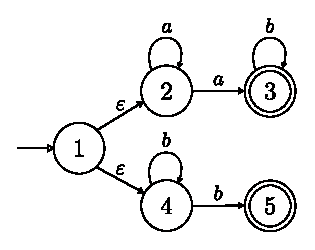
\includegraphics[width=0.4\textwidth]{obrazky-figures/ka_diagram_prechodu.eps}
        \caption{Přechodový diagram KA $M$ z~Příkladu \ref{example_ka}.}
        \label{fig_ka_prechodovy_diagram}
    \end{figure}
\end{example}

\section{Zásobníkový automat}\label{kap_zasobnikovy_automat}
Zásobníkový automat je rozšíření konečného automatu, popsaného v~Definici \ref{def_konecny_automat}, o~zásobník.
Zásobník slouží jako paměťové médium, na které si automat může ukládat informace v~podobě symbolů zásobníkové abecedy.
Následující definice převzaty z~\cite{meduna2023automata, TIN-opora}.
\begin{definition}\label{def_zasobnikovy_automat}
    \emph{Zásobníkový automat} (ZA) je sedmice 
    \begin{center}
        $M = (Q, \Sigma, \Gamma, R, s, S, F)$,
    \end{center}
    kde:
    \begin{itemize}
        \item $Q, \Sigma, s, F$ jsou definovány stejně jako v~Definici \ref{def_konecny_automat},
        \item $\Gamma$ je konečná zásobníková abeceda,
        \item $R$ je konečná relace $R \subseteq \Gamma \times Q \times (\Sigma \cup \{\varepsilon\}) \times \Gamma^* \times Q$ nazývána množinou pravidel ZA,
        \begin{itemize}[label=$\circ$]
            \item každé pravidlo $(A, q, a, w, p)$ může být zapsáno ve tvaru $Aqa \rightarrow wp$, kde $A \in \Gamma,$ $q, p \in Q,\; a \in \Sigma \cup \{\varepsilon\},\; w \in \Gamma^*$ \cite{meduna2017modely},
        \end{itemize}  
        \item $S \in \Gamma$ je počáteční symbol na zásobníku.
    \end{itemize}
\end{definition}

\begin{convention}
    Zásobníkové automaty budou dále značeny zkráceně ZA.
\end{convention}

\begin{definition}\label{def_konfigurace_za}
    Nechť $M = (Q, \Sigma, \Gamma, R, s, S, F)$ je ZA.\\
    Konfigurací ZA nazveme trojici
    \begin{equation*}
        (\alpha, q, w) \in \Gamma^* \times Q \times \Sigma^*, 
    \end{equation*}
    kde
    \begin{itemize}
        \item $\alpha$ je obsah zásobníku,
        \item $q$ je aktuální stav automatu (\emph{řídící jednotky}),
        \item $w$ je doposud nepřečtená část vstupního řetězce, jehož první symbol je aktuálně pod čtecí hlavou.
        Pokud $w = \varepsilon$, všechny symboly byly ze vstupní pásky již přečteny.
    \end{itemize}
    Nechť $X_M$ reprezentuje množinu všech konfigurací ZA $M$.
\end{definition}

\begin{definition}\label{def_prechod_za}
    Nechť $M = (Q, \Sigma, \Gamma, R, s, S, F)$ je ZA.\\
    Přechod ZA je binární relace definována nad množinou konfigurací (podobně jako v~Definici \ref{def_prechod_ka}) v~podobě
    \begin{equation*}
        \beta\; \vdash \chi,
    \end{equation*}
    kde $\beta = (uA, q, av),\; \chi = (uw, p, v)$ a~$Aqa \rightarrow wp \in R$.
    Symbolem $A$ je reprezentován vrchol zásobníku a~symbol $a$ nechť reprezentuje aktuální symbol pod čtecí hlavou.
    Pokud $w = \varepsilon$, pak se pouze vyjme $A$ ze zásobníku bez náhrady.
    Relace $\vdash^n,\; \vdash^+,\; \vdash^*$ jsou opět $n$-tou mocninou relace, tranzitivním a~reflexivně-tran\-zi\-tiv\-ním uzávěrem.
\end{definition}
Oproti klasickým KA se při přechodu musí pracovat se zásobníkem, ze kterého se vyjme symbol $A$, namísto něj se vloží symbol $w$.

Automat $M$ přijímá řetězec právě tehdy, když sekvencí přechodů dosáhne koncového stavu.
\begin{definition}\label{def_jazyk_za}
    Nechť $M = (Q, \Sigma, \Gamma, R, s, S, F)$ je ZA.\\
    Jazyk přijímaný $M$ je
    \begin{equation*}
        L(M) = \{w : w \in \Sigma^*,\; Ssw \vdash^* uf,\; u \in \Gamma^*,\; f \in F\}.
    \end{equation*}
\end{definition}

\begin{example}\label{example_za}
    Nechť $M = (\{s, f\}, \{a, b\}, \{S, a\}, R, s, S, \{f\})$ je ZA a 
    \begin{equation*}
        R = \{Ssa \rightarrow as,\; asa \rightarrow aas,\; asb \rightarrow f,\; afb \rightarrow f\}.
    \end{equation*}
    Počáteční konfigurace nechť je $(S, s, aaabbb)$.
    Přechody $M$ budou vypadat následovně:
    \begin{alignat*}{2}
        (S, s, aaabbb) &\vdash (a, s, aabbb) \quad && [Ssa \rightarrow as] \\
                       &\vdash (aa, s, abbb) \quad && [asa \rightarrow aas] \\
                       &\vdash (aaa, s, bbb) \quad && [asa \rightarrow aas] \\
                       &\vdash (aa, f, bb) \quad   && [asb \rightarrow f] \\ 
                       &\vdash (a, f, b) \quad      && [afb \rightarrow f] \\
                       &\vdash (\varepsilon, f, \varepsilon) \quad && [afb \rightarrow f]
    \end{alignat*}
    Je dobré dodat, že zásobníkové automaty, podobně jako konečné automaty, mohou být také reprezentovány graficky.
    Díky komplikaci zásobníkem se používá především přechodový diagram.
    \begin{figure}[ht]
        \centering
        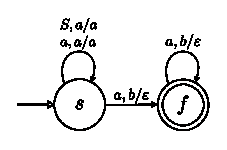
\includegraphics[width=0.4\textwidth]{obrazky-figures/za_diagram_prechodu.eps}
        \caption{Diagram přechodů ZA $M$ z~příkladu \ref{example_za}.}
        \label{fig_diagram_prechodu_za}
    \end{figure}
    Z~výčtu pravidel, přechodového diagramu a~kroků přijímání řetězce je vidět, že přijímaný jazyk ZA $M$ je $a^nb^n,\; n \geq 1$.
\end{example}

\subsection*{Rozšířený zásobníkový automat}\label{kap_rozsireny_ZA}
Rozšířené zásobníkové automaty reprezentují přirozené rozšíření klasických ZA, které na zásobníku mohou pracovat pouze s~jeho vrcholem.
Rozšířené zásobníkové automaty mohou provádět expanzi symbolů na zásobníku v~libovolné hloubce, jinak pracují indenticky.
Text a~definice v~této kapitole převzaty z~\cite{meduna2023automata, meduna_zemek_2014}, není-li řečeno jinak.

\begin{definition}\label{def_rza}
    \emph{Rozšířený zásobníkový automat} (RZA) je sedmice
    \begin{center}
        $M = (Q, \Sigma, \Gamma, R, s, S, F)$,
    \end{center}
    kde:
    \begin{itemize}
        \item $Q, \Sigma, s, S, F$ jsou definovány stejně jako u~klasických ZA v~Definici \ref{def_zasobnikovy_automat},
        \item $\Gamma$ je zásobníková abeceda, $\mathbb{N},\; Q,$ a~$\Gamma$ jsou navzájem disjunktní, $\Sigma \subseteq \Gamma$ a~$\Gamma \setminus \Sigma$ obsahuje speciální symbol $\#$ (\emph{spodní symbol}), který je považován za dno zásobníku, 
        \item $R$ je konečná relace
        \begin{alignat*}{-1}
             &(\mathbb{N} \times Q \,\times \,&& (\Gamma \setminus (\Sigma \cup \{\#\})) &&\times Q \times (\Gamma \setminus \{\#\})^+) \;\cup \\
             &(\mathbb{N} \times Q \,\times \,&& \{\#\} &&\times Q \times (\Gamma \setminus \{\#\})^*\{\#\}),
        \end{alignat*}
        místo uspořádané pětice $(m, q, A, p, v) \in R$ píšeme $mqA \rightarrow pv \in R$ a~$R$ nazýváme množinou pravidel.
        \begin{itemize}[label=$\circ$]
            \item Z definice $R$ lze vidět, že jsou dva typy přechodových pravidel, dají se zapsat ve tvaru
            \begin{align*}
                mqA  &\rightarrow pv,\\
                mq\# &\rightarrow pv\# \; \cite{meduna_rgd_pda}.
            \end{align*}
            O~jejich použití a~rozdílech je psáno v~Definici \ref{def_prechod_rza}.
        \end{itemize}
    \end{itemize}
\end{definition}

\begin{convention}
    Rozšířené zásobníkové automaty budou dále označeny zkratkou RZA.
\end{convention}

Přechody RZA pracují, stejně jako přechody ZA, nad konfiguracemi.
Konfigurace jsou podobné těm u~klasických ZA, nicméně stav zásobníku musí končit symbolem $\#$ a~zbytek řetězce na zásobníku jej nesmí obsahovat. 
\begin{definition}\label{def_konfigurace_za}
    Nechť $M = (Q, \Sigma, \Gamma, R, s, S, F)$ je RZA.\\
    Konfigurací RZA nazveme trojici
    \begin{equation*}
        (q, w, \alpha) \in Q \times \Sigma^* \times (\Gamma \setminus \{\#\})^*\{\#\}.
    \end{equation*}
    Nechť $X_M$ reprezentuje množinu všech konfigurací RZA $M$.
\end{definition}

Další podobnost je práce s~řetězci abedecedy $\Sigma$ a~s~pravidly při přechodech. 
Jediná změna od klasických ZA již byla zmíněna na začátku této kapitoly\,--\,při přechodech se na vrcholu zásobníku mohou měnit celé řetězce.

\begin{definition}\label{def_prechod_rza}
    Nechť $M = (Q, \Sigma, \Gamma, R, s, S, F)$ je RZA a~$\beta,\; \chi \in X_M$ jeho konfigurace.\\
    $M$ vyjme (anglicky \emph{pops}) ze zásobníku symbol a~přejde z~konfigurace $\beta$ do konfigurace $\chi$ za přečtení symbolu vstupní pásky, symbolicky zapsáno
    \begin{equation*}
        \beta\, \prescript{}{p}{\vdash}\; \chi,
    \end{equation*}
    pokud konfigurace jsou ve tvaru $\beta = (q, au, az),\; \chi = (q, u, z),\; a \in \Sigma$, $u \in \Sigma^*$, ${z \in \Gamma^*}$.
    $M$ rozšíří (anglicky \emph{expands}) symbol na zásobníku a~přejde z~konfigurace $\beta$ do konfigurace $\chi$ za přečtení symbolu ze vstupní pásky, symbolicky zapsáno
    \begin{equation*}
        \beta\, \prescript{}{e}{\vdash}\; \chi,
    \end{equation*} 
    pokud konfigurace jsou ve tvaru $\beta = (q, w, uAz),\; \chi = (p, w, uvz)$ a~zároveň $mqA \rightarrow pv \in R$; $q, p \in Q$, $w \in \Sigma^*$, $A \in \Gamma$, $u, v, z \in \Gamma^*$; $m$ je hloubka symbolu $A$ v~zásobníku, respektive $u$ obsahuje $m-1$ \emph{nevstupních} symbolů (symboly $a$, pro které platí $\{a\, :\, a \in \Gamma \setminus \Sigma\}$). 
    Pro ilustraci, že automat udělá přechod $\beta\, \prescript{}{e}{\vdash}\; \chi$ podle pravidla $mqA \rightarrow pv$, píšeme
     \begin{equation*}
        \beta\, \prescript{}{e}{\vdash}\; \chi \ \; [mqA \rightarrow pv].
    \end{equation*}
    $M$ udělá \emph{přechod} z~$\beta$ do $\chi$, psáno
    \begin{equation*}
        \beta\, \vdash\, \chi
    \end{equation*}
    právě tehdy, když $M$ udělá vyjmutí symbolu $\beta\, \prescript{}{p}{\vdash}\; \chi$ nebo expanzi symbolu $\beta\, \prescript{}{e}{\vdash}\; \chi$.
    Tranzitivní uzávěry $\prescript{}{p}{\vdash^+}, \prescript{}{e}{\vdash^+}$, reflexivně-tranzitivní uzávěry $\prescript{}{p}{\vdash^*}, \prescript{}{e}{\vdash^*}$ a~$n$-té mocniny $\prescript{}{p}{\vdash^n}, \prescript{}{e}{\vdash^n}$ jsou definovány standardně.
\end{definition}
Ilustrace obou typů přechodů jsou zobrazeny na obrázcích \ref{fig_p-prechod_rza} a~\ref{fig_e-prechod_rza}.

\begin{figure}[ht]
    \centering
    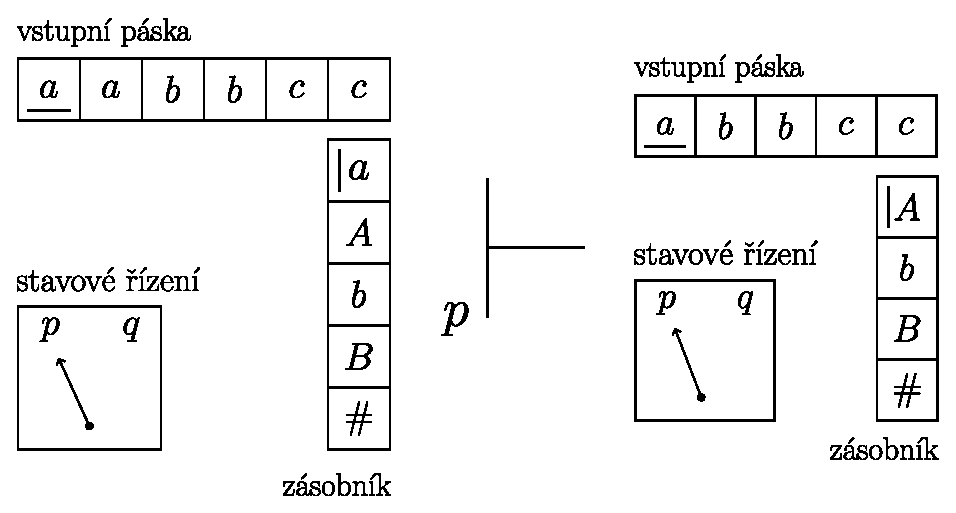
\includegraphics[width=0.7\textwidth]{obrazky-figures/rza_pop.eps}
    \caption{Ilustrace p-přechodu RZA (inspirace čerpána v~\cite{meduna_rgd_pda}).}
    \label{fig_p-prechod_rza}
\end{figure}

\begin{figure}[ht]
    \centering
    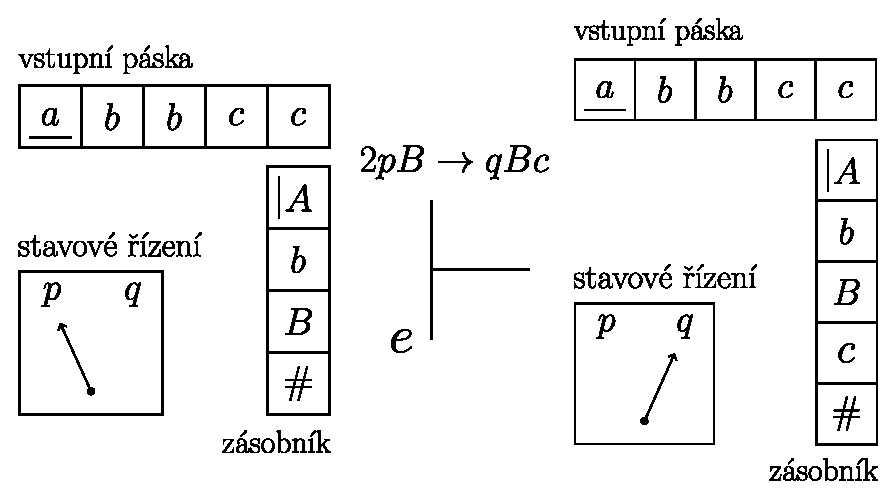
\includegraphics[width=0.7\textwidth]{obrazky-figures/rza_expanze.eps}
    \caption{Ilustrace e-přechodu RZA (inspirace čerpána v~\cite{meduna_rgd_pda}).}
    \label{fig_e-prechod_rza}
\end{figure}

Pokud existuje $n \in \mathbb{N}$ takové, že pro všechna pravidla $M$ platí, že jejich hloubka je maximálně rovna $n$, pak říkáme, že $M$ je hloubky maximálně $n$, zapsáno $\prescript{}{n}{M}$.

\begin{definition}\label{def_jazyk_rza}
    Nechť $\prescript{}{n}{M} = (Q, \Sigma, \Gamma, R, s, S, F)$ je RZA hloubky $n \in \mathbb{N}$. \\
    Jazyk přijímaný automatem $M$ je
    \begin{equation*}
        L(\prescript{}{n}{M}) = \{w \in \Sigma^*: (s, w, S\#) \vdash^* (f, \varepsilon, \#) \text{ v } \prescript{}{n}{M},\; f \in F\}.
    \end{equation*}
\end{definition}

Tyto jazyky jsou přijímané vyprázdněním zásobníku a~zároveň přechodem do koncového stavu automatu.
Dále existují jazyky přijímané RZA pouze vyprázdněním zásobníku, přičemž automat se nemusí dostat do koncového stavu.

\begin{definition}\label{def_jazyk_rza_empty}
    Nechť $\prescript{}{n}{M} = (Q, \Sigma, \Gamma, R, s, S, F)$ je RZA hloubky $n \in \mathbb{N}$. \\
    Jazyk přijímaný automatem M vyprázdněním zásobníku je
    \begin{equation*}
        E(\prescript{}{n}{M}) = \{w \in \Sigma^* : (s, w, S\#) \vdash^* (q, \varepsilon, \#) \text{ v~}\prescript{}{n}{M},\; q \in Q\}.
    \end{equation*}
\end{definition}

\begin{example}\label{example_rza}
    Nechť $\prescript{}{2}{M} = (\{s, q, p, f\}, \{a, b, c\}, \Sigma \cup \{A, S, \#\}, R, s, S, \{f\})$, kde $R$ je
    \begin{alignat*}{3}
        & 1sS \rightarrow qAA, \qquad \qquad && 1qA \rightarrow fab, \qquad \qquad && 1fA \rightarrow fc, \\
        & 1qA \rightarrow paAb, \qquad \qquad && 2pA \rightarrow qAc. \qquad \qquad &&
    \end{alignat*}
    Mějme počáteční konfiguraci $(s, aabbcc, S\#)$.
    $M$ udělá nejdříve dvakrát expanzi\,--\,jednou expanduje startovací symbol na $AA$, přičemž $A$ není vstupní symbol, takže expanze proběhne podruhé.
    \begin{alignat*}{2}
        (s, aabbcc, S\#)\, &\prescript{}{e}{\vdash}\; (q, aabbcc, AA\#) \quad && [1sS \rightarrow qAA] \\
                           &\prescript{}{e}{\vdash}\; (p, aabbcc, aAbA\#) \quad && [1qA \rightarrow paAb] \\
    \end{alignat*}
    Na aktuální konfiguraci je vidět, že na vrcholu zásobníku i~aktuálně čtený symbol je $a$.
    $M$ tento symbol vyjme.
    \begin{equation*}
        (p, aabbcc, aAbA\#)\, \prescript{}{p}{\vdash}\; (p, abbcc, AbA\#)
    \end{equation*}
    Následující krok bude znovu expanze, tentokrát hlouběji v~zásobníku.
    \begin{equation*}
        (p, abbcc, AbA\#)\, \prescript{}{e}{\vdash}\; (q, abbcc, AbAc\#) \quad [2pA \rightarrow qAc]
    \end{equation*}
    Dále přijímání řetězce probíhá stejným způsobem jako v předešlých krocích.
    \begin{alignat*}{2}
        (q, abbcc, AbAc\#)\, &\prescript{}{e}{\vdash}\; (q, abbcc, abbAc\#) \quad && [1qA \rightarrow fab] \\
                             &\prescript{}{p}{\vdash}\; (f, bbcc, bbAc\#) \quad && \\
                             &\prescript{}{p}{\vdash}\; (f, bcc, bAc\#) \quad && \\
                             &\prescript{}{p}{\vdash}\; (f, cc, Ac\#) \quad && \\
                             &\prescript{}{e}{\vdash}\; (f, cc, cc\#) \quad && [1fA \rightarrow fc] \\ 
                             &\prescript{}{p}{\vdash}\; (f, c, c\#) \quad && \\
                             &\prescript{}{p}{\vdash}\; (f, \varepsilon, \#) \quad &&
    \end{alignat*}
\end{example}

\chapter{Gramatické systémy}\label{kap_GS}
Veškeré definice a znalosti použité v~této kapitole převzaty z~\cite{CDGS, PCGS, Handbook-Of-Formal-Languages-2}, není-li řečeno jinak.

\section{Kooperující distribuované gramatické systémy}\label{kap_CDGS}

Kooperující distribuovaný (\emph{cooperating distributed}) gramatický systém stupně~\emph{n}~je systém gramatik, které mezi sebou sdílejí množinu neterminálů i~terminálů a~startovací symbol.
Spolupracují mezi sebou předáváním řízení derivace aktuálně zpracovávaného řetězce dle pravidel nastaveného \emph{derivačního režimu}.

\begin{definition}\label{def_cdgs}
\text{Kooperující distribuovaný gramatický systém je $(n+3)$-tice}
\begin{center}
    $\Gamma = (N, T, S, P_1, \ldots ,P_n)$,
\end{center}
kde:
\begin{itemize}
    \item $N$, $T$, a $S$ jsou definovány stejně jako v~Definici \ref{def_bkg},
    \item $P_i$ je konečná množina pravidel ve tvaru $A\rightarrow \alpha$, kde pravidla jsou definována stejně jako v~Definici \ref{def_bkg}, nazývaná \emph{komponentou} systému, $i \in \{1, \ldots, n\}$,
    \item $i$-tá gramatika systému se zapisuje jako $G_i = (N,T,S,P_i)$
\end{itemize}   
\end{definition}

\begin{convention}
    Pro označení kooperujících distribuovaných gramatických systémů bude dále využito zkrácené \emph{CDGS}, případně \emph{CD gramatické systémy}.
\end{convention}

\subsection*{Derivační krok v~CDGS}
Notace derivačního kroku v~CDGS je
\begin{center}
    $\alpha \prescript{}{i}{\Rightarrow}^{f} \beta$.
\end{center}
Tento zápis znamená, že řetězec $\alpha \in (N \cup T)^{*}$ derivuje řetězec $\beta \in (N \cup T)^{*}$ v~$i$-té komponentě za použití \emph{derivačního režimu} $f$.

\subsubsection*{Derivační režimy}

Prvním příkladem je režim $*$, který byl v~Definici \ref{def_der_krok_refl_tranz} uveden pro bezkontextovou gramatiku a~princip v~CD gramatických systémech je podobný.
Při použití tohoto derivačního režimu řetězec $\alpha \in (N \cup T)^*$ derivuje řetězec $\beta \in (N \cup T)^*$ v~libovolném počtu kroků v~$i$-té komponentě, zapsáno $\alpha \prescript{}{i}{\Rightarrow}^{*} \beta$.
Je možné předat řízení derivace jiné komponentě i~v~případě, že ve stejné komponentě lze s~derivací stejného řetězce pokračovat.

Podobným příkladem je režim \emph{ukončovací}, který spočívá v~nutné derivaci řetězce v~dané komponentě, dokud je to možné. Značí se písmenem \emph{t}. Jsou dvě nutné podmínky, aby $\beta$ bylo derivovatelné z~$\alpha$ v~komponentě $G_i$ režimem \emph{t}.
\begin{enumerate}
    \item $\alpha \prescript{}{i}{\Rightarrow}^{*} \beta$\,--\,v~dané komponentě lze posloupností derivačních kroků získat řetězec $\beta$ z~řetězce $\alpha$,
    \item $\beta \prescript{}{i}{\nRightarrow}\; \gamma$ pro všechna $\gamma \in (N \cup T)^{*}$\,--\,ve stejné komponentě nelze nalézt další pravidlo, které by derivovalo $\beta$.
\end{enumerate}
Jinými slovy, pokud můžeme z~aktuálního řetězce v~aktuální komponentě odvodit řetězec nový, \emph{musí} se s~derivací v~této komponentě pokračovat. 

Další derivační režimy jsou například
\begin{itemize}
    \item alespoň \emph{k}~derivací, tedy $\alpha \prescript{}{i}{\Rightarrow}^{\geq k}\; \beta$,
    \item nejvíce \emph{k}~derivací, tedy $\alpha \prescript{}{i}{\Rightarrow}^{\leq k}\; \beta$,
    \item právě \emph{k}~derivací, tedy $\alpha \prescript{}{i}{\Rightarrow}^{=k}\; \beta$,
\end{itemize}
kde $k \in \mathbb{N} \cup \{0\}$ a $i$ symbolizuje $i$-tou komponentu gramatického systému.
Tyto režimy mohou být reprezentovány jako množina, což pomůže definovat další pojmy v~následující podkapitole o~generovaném jazyce.
\begin{definition}\label{def_der_rezimy}
    Nechť $k\in \mathbb{N}$ a $*$, $t$ představují derivační režimy. \\
    Potom množina
    \begin{equation*}
        D = \{*, t\} \cup \{\leq k, \geq k, =k\}
    \end{equation*}        
    reprezentuje derivační režimy použitelné v~CD gramatických systémech.
\end{definition}

\subsection*{Jazyk generovaný CD gramatickým systémem}
Než bude definován samotný jazyk, je vhodné definovat pomocnou množinu, která reprezentuje \emph{možné derivace} z~řetězců.
\begin{definition}\label{def_mozne_derivace}
    Nechť $\Gamma = (N, T, S, P_1, \ldots, P_n)$. \\  
    Potom 
    \begin{equation*}
        F(G_j,\beta,f)=\{\beta : \alpha \prescript{}{j}{\Rightarrow^{f}}\beta\},\; j \in \{1, \ldots, n\},\; f\in D,\; \alpha \in (N \cup T)^{*}
    \end{equation*}        
    je množina všech řetězců $v$ derivovatelných z~$u$ v~$j$-té komponentě za použití derivačního režimu $f$.
\end{definition}

\begin{definition}\label{def_generovany_jazyk}
    Nechť $\Gamma = (N, T, S, P_1, \ldots, P_n)$. \\  
    Jazyk generovaný systémem $\Gamma$ za derivačního režimu $f$ je 
    \begin{align*}
         L_f(\Gamma) = \{&w \in T^*: \text{ existují } \alpha_0, \alpha_1,\ldots, \alpha_m \text{ takové, že } \alpha_k \in F(G_{j_{k}},\alpha_{k-1}, f),\\
         &k \in \{1, \ldots, m\},\;j_k \in \{1, \ldots, n\},\; \alpha_0 = S,\;\alpha_m = w \text{ pro } m \geq 1\}.
    \end{align*}        
\end{definition} 

Výsledný řetězec $w$, který vznikl postupnou derivací startovacího symbolu $\alpha_0$.
Měl několik mezikroků, které jsou reprezentovány řetězci $\alpha_1, \ldots, \alpha_{m-1}$.
Každý řetězec $\alpha_k$, kde $k \in \{1, \ldots, m\}$ byl zderivován z~řetězce $\alpha_{k-1}$ v~komponentě $G_{j_{k}}$, kde $j_k \in \{1, \ldots, n\}$, za derivačního režimu $f$.

\begin{example}
    Nechť $\Gamma = (\{S, A\}, \{a\}, S, P_1, P_2, P_3)$, kde $P_1 = \{S \rightarrow AA\}$, $P_2 = \{A \rightarrow S\}$, $P_3 = \{A \rightarrow a\}$.
    Nechť $f = t$, $\Gamma$ pracuje na ukončovacím derivačním režimu.

    Počáteční řetězec je počáteční symbol, tedy $S$. 
    Je pouze jedna možnost, jak $S$~přepsat, a~to použitím pravidla z~$P_1$, $S \rightarrow AA$.
    \begin{equation*}
        S \rightarrow AA \quad [S \rightarrow AA]
    \end{equation*}
    Díky tomu, že v~komponentě $P_1$ už neexistuje pravidlo, kterým by mohla derivace dále pokračovat, řízení derivace je předáno komponentě jiné.
    Aktuálně zpracovávaný řetězec je $AA$.
    Komponenty $P_1$ a~$P_2$ mají pravidla pro přepsání neterminálu $A$.
    Při použití derivačního režimu \emph{t} je zřejmé, že celý řetězec bude přepisovat pouze jedna komponenta.
    Při předání komponentě $P_3$ je řetězec přepsán na $aa$,
    \begin{alignat*}{-1}
        AA \rightarrow&&\; aA \quad &&[A \rightarrow a] \\
        aA \rightarrow&&\; aa \,\quad &&[A \rightarrow a]
    \end{alignat*}
    komponenta $P_2$ stejný řetězec přepíše na $SS$.
    \begin{alignat*}{-1}
        AA  \rightarrow&&\; SA && \quad [A~\rightarrow S] \\
        SA  \rightarrow&&\; SS && \quad [A~\rightarrow S] 
    \end{alignat*}
    \begin{alignat*}{-1}
         SS \rightarrow&&\; AAS  \hphantom{A} \quad  &&[S \rightarrow AA] \\ 
        AAS \rightarrow&&\; AAAA \quad &&[S \rightarrow AA]
    \end{alignat*}
    Ze startovacího symbolu dostaneme buď terminál $a$ nebo dva startovací symboly.
    To znamená, že pokaždé, kdy se $AA$ přepíše na $SS$, počet terminálů $a$ se zdvojnásobí.
    Jazyk generovaný systémem $\Gamma$ za derivačního režimu \emph{t}, $L(\Gamma)_t = \{a^{2^n},$ $n \geq 1 \}$.
\end{example}

\subsection*{Klasifikace skupin CD jazyků}
CD jazyky jsou jazyky, které jsou generovány CD gramatickými systémy.
Tyto jazykové rodiny se rozdělují podle různých typů použitých CDGS.
Jejich označení je
\begin{center}
    $CD^y_x(f)$,
\end{center}
kde:
\begin{itemize}
    \item $y$ určuje použití $\varepsilon$-pravidel: 
    \begin{itemize}[label=$\circ$]
        \item $y = \varepsilon$\,--\,$\varepsilon$-pravidla v~komponentách jsou povolena,
        \item $y$ chybí\,--\,$\varepsilon$-pravidla se v~komponentách nemohou vyskytovat,
    \end{itemize}
    \item $x$ je stupeň gramatického systému:
    \begin{itemize}[label=$\circ$]
        \item $n, n \geq 1$\,--\,gramatický systém může obsashovat maximálně $n$~komponent,
        \item $\infty$\,--\,gramatický systém nemá omezen počet komponent,
    \end{itemize}
    \item $f$ je derivační režim, $f \in D$.
\end{itemize}
\begin{example}
    $CD^\varepsilon_6 (t)$ je rodina jazyků generována CD gramatickými systémy s~maximálně šesti komponentami, povolenými $\varepsilon$-pravidly a~pracujícími nad ukončovacím režimem. 
\end{example}

\subsection*{Hybridní CD gramatické systémy}
Hybridní CD gramatické systémy nabízí možnost definovat derivační režim samostatně pro jednotlivé komponenty systému.
\begin{definition}
    \emph{Hybridní CDGS} je n-tice $\Gamma = (N, T, S, (P_1, f_1), \ldots, (P_n, f_n))$, kde:
    \begin{itemize}
        \item $N, T, P_i, S$ jsou definovány stejně jako v~klasických CDGS v~Definici \ref{def_cdgs},
        \item $f_i$ je derivační režim $i$-té komponenty, $f_i \in D$ pro všechna $i \in \{1, \ldots, n\}$.
    \end{itemize}
\end{definition}

Jazyk generovaný těmito gramatickými systémy je velmi podobný jazykům generovaným klasickými CDGS.
Jediný rozdíl je v~použití derivačního režimu příslušné komponenty, který je v~definici označen jako $f_{j_k}$, místo společného derivačního režimu pro celý gramatický systém.
\begin{definition}
    Nechť $\Gamma = (N, T, S, (P_1, f_1), \ldots, (P_n, f_n))$.\\
    Jazyk generovaný systémem $\Gamma$,
    \begin{align*}
        L(\Gamma) = \{&w \in T^*: \text{existují } \alpha_0, \alpha_1,\ldots, \alpha_n \text{ takové, že } \alpha_k \in F(G_{j_k}, \alpha_{k-1}, f_{j_k}),\\
        &k \in \{1, \ldots, m\}, j_k \in \{1, \ldots, n\}, \alpha_0 = S, \alpha_m = w \text{ pro } m \geq 1\}.
    \end{align*}
\end{definition}

Zápis jazykových skupin generovaných hybridními CDGS je
\begin{center}
    $X\,CD^y_{x, v}(f) $, 
\end{center}
kde:
\begin{itemize}
    \item $x, y, f$ jsou definovány stejně jako u~nehybridních CDGS,
    \item $v$ je nepovinné omezení počtu pravidel v~komponentách:
    \begin{itemize}[label=$\circ$]
        \item \emph{m}\,--\,každá komponenta $P_i, i \in \{1, \ldots, n\}$ obsahuje nejvíce $m$ pravidel, $m \geq 1$,
        \item $\infty$, chybí\,--\, maximální počet pravidel pro komponenty není omezen,
    \end{itemize}
    \item $X$ určuje determinismus gramatického systému:
    \begin{itemize}[label=$\circ$]
        \item $D$\,--\,gramatický systém je deterministický, tedy pro každé $A \rightarrow u, A \rightarrow w \in P_i$, $i \in \{1, \ldots, n\}$ platí, že $u = w$.
        Jinými slovy, pro všechny neterminály platí, že pro jejich přepis neexistují pravidla (ve \emph{všech} komponentách), která by měla různé pravé strany.
        \item \emph{nic}\,--\,gramatický systém je nedeterministický.
        To znamená, že v~\emph{každé} komponentě existuje pravidlo pro nějaký neterminál, které má různé pravé strany.
        \item $H$\,--\,gramatický systém je hybridní a~obsahuje alespoň jednu nedeterministickou komponentu a~jednu deterministickou komponentu.
        Nezapisuje se derivační režim, který je určen samostatně pro každou komponentu. 
    \end{itemize}
\end{itemize}

\section{Paralelní komunikující gramatické systémy}
Paralelní komunikující (\emph{parallel communicating})\,--\,PC gramatický systém stupně $n$ je systém gramatik, v~němž každá začíná vlastním startovacím symbolem (\emph{axiomem}), které sdílí množinu neterminálů i~terminálů a~nově množinu komunikačních symbolů.
Komunikační symboly slouží ke komunikaci na vyžádání.
Kdykoliv se vyskytnou ve větné formě libovolné komponenty, proběhne \emph{komunikační krok} (také nazýván \emph{c-derivační krok}).

Komunikačních symbolů je stejné množství jako komponent v~PC gramatickém systému, $\{Q_1, \ldots, Q_n\}$, kde index symbolu $Q_i$ odkazuje na komponentu $P_i$ \cite{PCGS-chapter2}.
\begin{definition}
    Paralelní komunikující gramatický systém stupně $n, n \geq 1$ je $(n+3)$-tice
    \begin{center}
        $\Gamma = (N, K, T, (S_1, P_1), \ldots, (S_n, P_n))$,
    \end{center}
    kde:
    \begin{itemize}
        \item $N, T$ jsou definovány stejně jako u~bezkontextových gramatik v~Definici \ref{def_bkg},
        \item $K = \{Q_1, \ldots, Q_n\}$ je množina komunikačních symbolů ($N, K, T$ jsou navzájem disjunktní); index $i$ komunikačního symbolu $Q_i$ koresponduje s~indexem $i$-té komponenty,
        \item $P_i,\; i \in \{1, \ldots, n\}$ je množina pravidel nazývané komponenty, stejně jako u~CD gramatických systémů v~Definici \ref{def_cdgs},
        \item $i$-tá gramatika systému je konstrukt $G_i = (N \cup K, T, S_i, P_i),\; i \in \{1, \ldots, n\}$.
    \end{itemize}
\end{definition}

\begin{convention}
Pro označení paralelních komunikujících gramatických systémů bude dále využito zkrácené \emph{PCGS} nebo \emph{PC gramatické systémy}.
\end{convention}

\subsection*{Derivační kroky v~PCGS}

V~PC gramatických systémech existují dva druhy derivačního kroku, a~to \emph{g}-derivační krok a~\emph{c}-derivační krok.
První zmíněný slouží k~přímé derivaci řetězce v~rámci jedné komponenty bez zásahu komponent jiných a~druhý slouží pro vzájemnou pomoc při derivaci řetězce. 
PC gramatický systém \emph{vždy} preferuje c-derivační krok nad g-derivačním krokem.
Ten se provede pokaždé, obsahuje-li alespoň jeden z~řetězců $\alpha_i,\; i \in \{1, \ldots, n\}$ alespoň jeden komunikační symbol.

Derivační kroky pracují nad \emph{konfigurací} PCGS.
Následující definice převzata z~\cite{Various-communications-in-PC-grammar-systems}.
\begin{definition}
    Nechť $\Gamma = (N, K, T, (S_1, P_1), \ldots, (S_n, P_n))$ je PC gramatický systém.
    Potom n-tice
    \begin{equation*}
        (\alpha_1, \ldots, \alpha_n),\; \alpha_i \in (N \cup K \cup T)^*,\; i \in \{1 \ldots, n\}
    \end{equation*}
    se nazývá \emph{konfigurací} $\Gamma$. $(S_1, \ldots, S_n)$ je \emph{počáteční konfigurací} $\Gamma$.
\end{definition}
Nutná podmínka k~proběhnutí libovolného derivačního kroku je $\alpha_1 \notin T^*$.
Pokud tato situace nastane, už je vygenerována věta jazyka definovaného PCGS a~dále se s~kroky nepokračuje. 
Více v~Definici \ref{def_gener_jazyk_pcgs}.

\subsubsection*{g-derivační krok}\label{kap_g_der_krok}
Nechť $\Gamma = (N, K, T, (P_1, S_1), \ldots, (P_n, S_n))$ je PCGS a~$(\alpha_1, \ldots \alpha_n),\; (\beta_1, \ldots, \beta_n)$ jsou konfigurace $\Gamma$.
$\Gamma$ udělá g-derivační krok, formálně zapsáno
\begin{center}
    $(\alpha_1, \ldots, \alpha_n) \prescript{}{g}{\Rightarrow} (\beta_1, \ldots, \beta_n)$
\end{center}
pokud $alph(\alpha_i) \cap K = \emptyset$ a~zároveň:
\begin{itemize}
    \item $\alpha_i \Rightarrow \beta_i$ v~$G_i = (N, K, T, (S_i, P_i))$\,--\,$\beta_i$ je přímo derivován z~$\alpha_i$ v~gramatice $G_i$ (komponentě $P_i$), nebo
    \item $\alpha_i = \beta_i \in T^*$\,--\,$\alpha_i$ již je řetězcem terminálů
\end{itemize}   
pro všechna $i \in \{1, \ldots, n\}$.

\subsubsection*{c-derivační krok}\label{kap_c_der_krok}
Někdy taky nazýván \emph{komunikační krok}. Tento koncept umožňuje gramatikám spolupracovat a~vzájemně si mezi sebou měnit vygenerované řetězce pomocí komunikačních symbolů.
Algoritmus ukazující princip komunikačního kroku je následující:
\begin{algorithm}[h]
    \caption{c-derivační krok v~PCGS}
    \label{alg_c_der_krok}
    \begin{algorithmic}[1]
        \Input{konfigurace $(\alpha_1, \ldots, \alpha_n)$}
        \Output{konfigurace $(\beta_1, \ldots, \beta_n)$}
        \NewLine

        \ForAll{$i \in \{1, \ldots, n\}$}
            \State $\gamma_i \gets \alpha_i$
        \EndFor 
        \ForAll{$i \in \{1, \ldots, n\}$}
            \If{$alph(\alpha_i) \cap K \neq \emptyset$ \textbf{and} \textbf{foreach} $Q_j$ \textbf{in} $\alpha_i$: $alph(\alpha_j) \cap K = \emptyset$}
                \ForAll{$Q_j$ \textbf{in} $\alpha_i$} 
                    \State $\gamma_j \gets S_j$\Comment{vynecháno, pokud PCGS pracuje na nevracejícím se režimu}
                    \State zaměň $Q_j$ za $\alpha_j$ v~$\alpha_i$
                    \State $\gamma_i \gets \alpha_i$\Comment{$\alpha_i =$ řetězec, který vznikl o~krok zpět} 
                \EndFor
            \EndIf
        \EndFor
        \State proveď $(\alpha_1, \ldots, \alpha_n) \prescript{}{c}{\Rightarrow} (\beta_1, \ldots, \beta_n)$ s~$\beta_i = \gamma_i,\;i \in \{1, \ldots, n\}$ 
    \end{algorithmic}
\end{algorithm}

\subsection*{Přímá derivace v~PCGS}
\begin{definition}
    Konfigurace $(\alpha_1, \ldots, \alpha_n)$ přímo derivuje konfiguraci $(\beta_1, \ldots, \beta_n)$, zapsáno
    \begin{center}
        $(\alpha_1, \ldots, \alpha_n) \Rightarrow (\beta_1, \ldots, \beta_n)$
    \end{center} 
    právě tehdy, když
    \begin{center}
        $(\alpha_1, \ldots, \alpha_n) \prescript{}{g}{\Rightarrow}\, (\beta_1, \ldots, \beta_n)$
    \end{center}
    nebo
    \begin{center}
        $(\alpha_1, \ldots, \alpha_n) \prescript{}{c}{\Rightarrow}\, (\beta_1, \ldots, \beta_n)$.
    \end{center}
\end{definition}

\subsection*{Jazyk generovaný PCGS}\label{def_gener_jazyk_pcgs}
Generování větné formy končí v~momentě, kdy první komponenta dosáhne řetězce terminálů a~na řetězcích ostatních komponent nezáleží.
\begin{definition}
    Nechť $\Gamma = (N, K, T, (P_1, S_1), \ldots, (P_n, S_n))$ je PCGS.
    Jazyk generovaný $\Gamma$ je stejný jako jazyk generovaný jeho první komponentou:
    \begin{align*}
        L_f(\Gamma) = \{&w \in T^*: (S_1, \ldots, S_n) \Rightarrow^*_f (w, \alpha_2, \ldots, \alpha_n),\\ 
        &for\ \alpha_i \in \{N \cup T \cup K\},\ i \in \{2, \ldots, n\},\ f \in \{r, nr\}\},
    \end{align*}
    kde $r$ a~$nr$ specifikuje \emph{vracející} nebo \emph{nevracející} PCGS.
\end{definition}

\subsection*{Vracející a nevracející se režim}
Pokud PC gramatický systém pracuje na vracejícím se režimu, potom komponenty, které v~rámci komunikačního kroku poslaly svůj řetězec jiným komponentám, generují řetězec od svého axiomu.
Při nevracejícím se režimu komponenty pokračují ve zpracovávání aktuálního řetězce.

Tato skutečnost se projeví na samotném komunikačním kroku, u~kterého se vynechá přiřazení axiomu do řetězce $\gamma_j$\,--\,neprovede se krok na řádku 10 Algoritmu \ref{alg_c_der_krok}.

\subsection*{Centralizované PCGS}
Centralizované PC gramatické systémy mají tu vlastnost, že pouze první komponenta (nazývaná \emph{master}) systému může generovat komunikační symboly a~tím žádat ostatní komponenty o~řetězce.
Řeší jeden z~možných případů uváznutí, kdy komponenty v~cyklu zavádějí komunikační symboly a~donekonečna se provádí stejná sekvence komunikačních kroků. 

\begin{definition}
    Nechť $\Gamma = (N, K, T, (S_1, P_1), \ldots, (S_n, P_n))$ je PCGS.
    Pokud pouze $P_1$ může uvést komunikační symboly, formálně
    \begin{center}
        $P_i \subseteq (N \cup T)^* \times (N \cup T)^*$ pro $i \in \{2, \ldots, n\}$,
    \end{center}
    potom $\Gamma$ je centralizovaný PC gramatický systém.
    Jinak je necentralizovaný.
\end{definition}

\subsection*{Příklady}
V~prvním příkladu bude pouze demonstrován princip obou derivačních kroků na systému, který generuje jen velmi omezený jazyk.
\begin{example}
    Nechť $\Gamma = (\{S_1, S_2, S_3\},$ $\{Q_3\},$ $\{a, b\},$ $(S_1, \{S_1 \rightarrow Q_3\}),$ $(S_2, \{S_2 \rightarrow a\}),$ $(S_3, \{S_3 \rightarrow b\}))$ je PCGS.
    Počáteční konfigurace $\Gamma$ je zřejmě $(S_1, S_2, S_3)$.
    Víme, že PC gramatické systémy \emph{vždy} preferují c-krok nad g-krokem, je-li to možné.
    Nutná podmínka je, aby alespoň jeden z~řetězců v~aktuální konfiguraci obsahoval alespoň jeden komunikační symbol, což aktuálně není splněno.
    $\Gamma$ tedy udělá g-krok.
     \begin{equation*}
    (S_1, S_2, S_3) \prescript{}{g}{\Rightarrow}\, (Q_3, a, b)
     \end{equation*}
     Nyní je v~konfiguraci komunikační symbol, což indikuje, že bude následovat komunikační krok.
     Při postupu podle Algoritmu~\ref{alg_c_der_krok} je postup následující:
     \begin{enumerate}
        \item Zavedení pomocných řetězců $\gamma_1 = Q_3$, $\gamma_2 = a$, $\gamma_3 = b$ podle řádků 4\,--\,6.
        \item Kontrola, zda řetězec $\alpha_i,\; i \in \{1, \ldots, n\}$ z~původní konfigurace obsahuje komunikační symboly (podmínka $alph(\alpha_i) \cap K \neq \emptyset$).
        \begin{itemize}[label=$\circ$]
            \item V~tomto příkladu splňuje podmínku pouze řetězec $\alpha_1$, který obsahuje $Q_3$.
        \end{itemize}
        \item Pokud $\alpha_i$ obsahuje komunikační symboly $Q_j$, z~každého se přečte index $j$ a~proběhne kontrola, zda všechny $j$-té řetězce konfigurace ($\alpha_j$) \emph{neobsahují} komunikační symboly.
        Tato část koresponduje s~podmínkou \textbf{foreach} $Q_j$ \textbf{in} $\alpha_i:$ $alph(\alpha_i) \cap K = \emptyset$ na řádku~8.
        \begin{itemize}[label=$\circ$]
            \item Řetězec $\alpha_1$ obsahuje jeden komunikační symbol $Q_3$, jehož index odkazuje na řetězec $\alpha_3$ z~aktuální konfigurace.
            Hodnota řetězce $\alpha_3$ je $b$, ten žádné další komunikační symboly neobsahuje.
        \end{itemize}
        \item Každý $Q_j$ v~$\alpha_i$ se nahradí za $\alpha_j$, pokud prošel podmínkou v~předchozím kroku.
        Zároveň se $\gamma_j$ nastaví na počáteční symbol $j$-té komponenty.
        Tyto kroky jsou v~Algoritmu \ref{alg_c_der_krok} na řádcích 9\,--\,12.
        \begin{itemize}[label=$\circ$]
            \item Komunikační symbol $Q_3$ bude v~$\alpha_1$ nahrazen řetězcem $b$ z~$\alpha_3$. Dále $\alpha_3 \gets S_3$ a~$\gamma_1 \gets \alpha_1$.
            Aktuálně $\gamma_1 = b,$ $\gamma_2 = a$, $\gamma_3 = S_3$. 
        \end{itemize}
        \item Proveď $(\alpha_1, \ldots, \alpha_n) \prescript{}{c}{\Rightarrow}\, (\beta_1, \ldots, \beta_n)$, kde $\beta_i = \gamma_i$ pro $i \in \{1, \ldots, n\}$.
        \begin{itemize}[label=$\circ$]
            \item Nová konfigurace $(\beta_1, \beta_2, \beta_3)$ bude stejná, jako pomocná konfigurace $(\gamma_1, \gamma_2, \gamma_3)$, a~to $(b, a, S_3)$.
        \end{itemize}
    \end{enumerate}
    $\Gamma$ provede komunikační krok z~$(Q_3, a, b)$ do $(b, a, S_3)$.
    \begin{center}
        $(Q_3, a, b) \prescript{}{c}{\Rightarrow}\, (b, a, S_3)$
    \end{center}
    Další kroky už $\Gamma$ provádět nebude, protože řetězec generovaný první komponentou je již řetězec terminálních symbolů.
    V~tomto příkladu byla použita sémantika vracejícího se PCGS, nicméně při použítí nevracejícího by jazyk vypadal stejně, jen výsledná konfigurace by se lišila v~řetězci $x_3$.
    \begin{equation*}
        L(\Gamma)_r = L(\Gamma)_{nr} = \{b\}
    \end{equation*}
\end{example}

Ve druhém příkladu bude demonstrováno několik derivačních kroků a~bude se zkoumat výsledný generovaný jazyk.
\begin{example}
    Nechť $\Gamma = (\{S_1, S_1', S_2, S_3\}, K, {a, b, c}, (S_1, P_1), (S_2, P_2), (S_3, P_3)),$ kde:
    \begin{align*}
        P_1 = \{S_1 &\rightarrow abc, S_1 \rightarrow a^2b^2c^2, S_1 \rightarrow aS_1', S_1 \rightarrow a^3Q_2, \\
                S_1' &\rightarrow aS_1', S_1' \rightarrow a^3Q_2, S_2 \rightarrow b^2Q_3, S_3 \rightarrow c\}, \\        
        P_2 = \{S_2 &\rightarrow bS_2\}, \\
        P_3 = \{S_3 &\rightarrow cS_3\}.
    \end{align*}
    Komunikační symboly může uvést pouze komponenta $P_1$, a~proto se jedná o~\emph{centralizovaný} PC gramatický systém.

    Počáteční konfigurace je $(S_1, S_2, S_3)$.
    $\Gamma$ může generovat konfiguraci $(aS_1', bS_2, cS_3)$ za použití pravidel $(S_1 \rightarrow aS_1', S_2 \rightarrow bS_2, S_3 \rightarrow cS_3)$.
    \begin{equation*}
        (S_1, S_2, S_3) \Rightarrow (aS_1', bS_2, cS_3)
    \end{equation*}
    Zřejmě při použití pravidel $(S_1' \rightarrow aS_1', S_2 \rightarrow bS_2, S_3 \rightarrow cS_3)$ $n$-krát po sobě je možné generovat konfigurace $(a^nS_1', b^nS_2, c^nS_3),\;n \geq 1$.
    \begin{equation*}
        (aS_1', bS_2, cS_3) \Rightarrow^* (a^nS_1', b^nS_2, c^nS_3)
    \end{equation*}
    Je vidět, že komponenty $P_2$ a~$P_3$ neustále používají ta samá pravidla, což je logické vzhledem k~jejich kardinalitě.
    Pro zjednodušení zápisu, při každém g-derivačním kroku bude zmíněno pouze pravidlo komponenty $P_1$, pravidla komponent $P_2$ a~$P_3$ budou vždy stejná.

    Z~konfigurace $(a^nS_1', b^nS_2, c^nS_3)$ se na rozdílný výsledek dá dostat pouze za použití pravidla $S_1' \rightarrow a^3Q_2$.
    \begin{equation*}
        (a^nS_1', b^nS_2, c^nS_3) \Rightarrow (a^{n+3}Q_2, b^{n+1}S_2, c^{n+1}S_3)
    \end{equation*} 
    Provedeme c-derivační krok a~zaměníme $Q_2$ za $\alpha_2$, nový $\alpha_2$ bude $S_2$, který je axiomem $G_2$.
    \begin{equation*}
        (a^{n+3}Q_2, b^{n+1}S_2, c^{n+1}S_3) \Rightarrow (a^{n+3}b^{n+1}S_2, S_2, c^{n+1}S_3)
    \end{equation*}
    Jediné pravidlo pro symbol $S_2$ v~komponentě $P_1$ je $S_2 \rightarrow b^2Q_3$.
    \begin{equation*}
        (a^{n+3}b^{n+1}S_2, S_2, c^{n+1}S_3) \Rightarrow (a^{n+3}b^{n+3}Q_3, bS_2, c^{n+2}S_3)
    \end{equation*}
    Zaměníme $Q_3$ za $\alpha_3$, nový $\alpha_3$ bude $S_3$, který je axiomem $G_3$.
    \begin{equation*}
        (a^{n+3}b^{n+3}Q_3, bS_2, c^{n+2}S_3) \Rightarrow (a^{n+3}b^{n+3}c^{n+2}S_3, bS_2, S_3)
    \end{equation*}
    Pro $S_3$ je v~$P_1$ také pouze jediné pravidlo, které se může aplikovat, a to $S_3 \rightarrow c$.
    \begin{equation*}
        (a^{n+3}b^{n+3}c^{n+2}S_3, bS_2, S_3) \Rightarrow (a^{n+3}b^{n+3}c^{n+3}, bbS_2, cS_3)
    \end{equation*}
     $\alpha_1$ je aktuálně řetězec terminálů, tudíž na něj nelze aplikovat žádné další pravidlo a~neobsahuje komunikační symboly.
     Je tedy generovaným jazykem pro $\Gamma$ ve vracejícím se režimu.
     Takto by vypadaly kroky pro nevracející se režim (konfigurace se začnou lišit od výskytu komunikačních symbolů):
     \begin{align*}
        (a^{n+3}Q_2, b^{n+1}S_2, c^{n+1}S_3) &\Rightarrow (a^{n+3}b^{n+1}S_2, b^{n+1}S_2, c^{n+1}S_3) \\
        &\Rightarrow (a^{n+3}b^{n+3}Q_3, b^{n+2}S_2, c^{n+2}S_3) \\
        &\Rightarrow (a^{n+3}b^{n+3}c^{n+2}S_3, b^{n+2}S_2, c^{n+2}S_3) \\
        &\Rightarrow (a^{n+3}b^{n+3}c^{n+3}, b^{n+3}S_2, c^{n+3}S_3)
     \end{align*}
     Je tedy zřejmé, že:
     \begin{equation*}
        L(\Gamma)_r = L(\Gamma)_{nr} = \{a^nb^nc^n,\; n \geq 1\}.
     \end{equation*}
\end{example}

\chapter{Syntaktická analýza}\label{kap_teorie_sa}
Tato kapitola se zabývá syntaktickou analýzou, která provádí kontrolu, zda je vstupní řetězec v~jazyce, který je formálně definován.
Ostatní části překladačů v~této práci nebudou rozebírány, nebude-li to vyžadovat kontext.
Celý proces překladu programů je podrobně popsán v~\cite{medunaElementsOfCompDesign}, odkud bude do této kapitoly převzato největší množství informací.

Syntax jazyka, ve kterém je napsán zdrojový kód, je nejčastěji popsána gramatikou (v~praxi nejčastěji bezkontextovou) jazyka s~konečnou množinou pravidel.
Pomocí těchto pravidel analyzátor zkontroluje, že posloupnost \emph{tokenů}, které jsou na vstupu od lexikálního analyzátoru, je korektní, podle použitých pravidel v~gramatice.
Při tomto procesu syntaktický analyzátor generuje \emph{derivační strom}, kde každý uzel a~jeho potomci reprezentují použité pravidlo.
Tento proces může probíhat \emph{shora dolů}, čímž se zabývá Kapitola \ref{kap_sa_shora_dolu}, případně \emph{zdola nahoru}, čímž se zabývá Kapitola \ref{kap_sa_zdola_nahoru}.
Tyto názvy jsou odvozeny od směru tvorby derivačního stromu, kdy analýza shora dolů postupuje od kořene k~listům, analýza zdola nahoru naopak.

Než se začneme zabývat těmito dvěma druhy syntaktické analýzy, pojďme si definovat pojmy \emph{nejlevější a nejpravější derivace} a~jejich sekvence.
\begin{definition}\label{def_nejlevejsi_nejpravejsi_der}
     Nechť $G = (N, T, P, S)$ je BKG, $r: A \rightarrow \alpha \in R$, $u \in T^*$, $\gamma \in (N \cup T)^*$. \\ 
     $G$ provede nejlevější derivační krok (\emph{leftmost derivation step}) z~$uA\gamma$ do $u\alpha\gamma$, podle pravidla $r$, symbolicky zapsáno
    \begin{equation*}
        uA\gamma\; \prescript{}{\scriptstyle lm}{\Rightarrow}\; u\alpha\gamma \; [r].
    \end{equation*}
    $G$ provede nejpravější derivační krok (\emph{rightmost derivation step}) z~$\gamma Au$ do $\gamma \alpha u$, podle pravidla $r$, symbolicky zapsáno
    \begin{equation*}
        \gamma Au\; \prescript{}{\scriptstyle rm}{\Rightarrow}\; \gamma \alpha u\; [r].
    \end{equation*}
\end{definition}

\begin{definition}\label{def_sekvence_nejl_nejpr_der}
    Nechť $G = (N, T, P, S)$ je BKG a~$\alpha_0, \alpha_1, \ldots, \alpha_n$ je sekvence řetězců, kde $\alpha_i \in (N \cup T)^*,$ $i \in \{1, \ldots, n\}$.\\
    Pokud $\alpha_{j-1}\; \prescript{}{\scriptstyle lm}{\Rightarrow}\; \alpha_j\; [r_j]$ v~$G$, kde $r_j \in R,\; j \in \{1, \ldots, n\}$, pak $G$ provede sekvenci nejlevějších derivačních kroků (\emph{nejlevější derivaci}) z~$\alpha_0$ do $\alpha_n$ podle $r_1, r_2, \ldots, r_n$, symbolicky zapsáno jako
    \begin{equation*}
        \alpha_0\; \prescript{}{\scriptstyle lm}{\Rightarrow}\; \alpha_n\; [r_1r_2\ldots r_n].
    \end{equation*} 
    Pokud $\alpha_{j-1}\; \prescript{}{\scriptstyle rm}{\Rightarrow}\; \alpha_j\; [r_j]$ v~$G$, kde $r_j \in R,\; j \in \{1, \ldots, n\}$, pak $G$ provede sekvenci nejpravějších derivačních kroků (\emph{nejpravější derivaci}) z~$\alpha_0$ do $\alpha_n$ podle $r_1, r_2, \ldots, r_n$, symbolicky zapsáno jako
    \begin{equation*}
        \alpha_0\; \prescript{}{\scriptstyle rm}{\Rightarrow}\; \alpha_n\; [r_1r_2\ldots r_n].
    \end{equation*}
\end{definition}
\todo{jestli zbude cas, napsat vlastnimi slovy, inspirace v \cite{medunaElementsOfCompDesign}, strana 83}


\section{Syntaktická analýza shora dolů}\label{kap_sa_shora_dolu}
Uvažujme BKG $G$.
Syntaktický analyzátor pracující shora dolů pro $G$ je reprezentován zásobníkovým automatem $M$, který je ekvivalentní k~$G$.
$M$ na svém zásobníku simuluje nejlevější derivace a~tvorbu derivačního stromu pro řetězce generované gramatikou $G$.
Aby tento model fungoval, musí $M$ obsahovat korespondující pravidla pro pravidla $G$ a~navíc mít pomocné pravidlo pro mazání terminálních symbolů z~vrchou zásobníku, pokud přečte stejný symbol ze vstupní pásky.

Pokud na vrcholu zásobníku je neterminál $A$, pak $M$ simuluje nejlevější derivační krok, který by udělala gramatika $G$ pomocí pravidla $r: A \rightarrow \alpha \in R$.
Provede expanzi pravidla nahrazením neterminálu $A$ z~vrcholu zásobníku za $reversal(\alpha)$. 

Existují dvě metody, a~to \emph{prediktivní syntaktická analýza} a~\emph{rekurzívní sestup}.
Více k~těmto metodám je psáno na konci této kapitoly.
\todo{doladit uvod tady po smazani bkg na za algoritmu}

\subsection*{Prediktivní množiny}
Předpokládejme BKG $G$ a~příslušný ZA $M$.
Dále předpokládejme, že existuje neterminál $A \in N$ takový, že pro něj existují dvě pravidla ve tvaru $A \rightarrow X\alpha$ a~$A \rightarrow Y\beta$.
$A$ musí být v~dalším kroku přepsán za nový řetězec a~zároveň musí být deterministicky zvolené pravidlo, které se použije.

K~deterministickému výběru slouží množina $Predict(A \rightarrow \gamma)$.
Pokud pravidla, která na levé straně mají neterminál $A$, mají množinu $Predict(A \rightarrow \gamma)$ navzájem disjunktní, pravidlo je zvoleno deterministicky.
Pro konstrukci množin $predict(A \rightarrow \gamma)$ je zapotřebí množin $Empty(\gamma)$, $First(\gamma)$ a~$Follow(A)$. 

Definice a~algoritmy v~této kapitole převzaty z~\cite{meduna2017sa-shora-dolu,kunda2022}, kde jsou popsány velmi intuitivně, nicméně ne tak podrobně, jako například v~\cite{medunaElementsOfCompDesign}.
Inspirace pro strukturu této kapitoly a~slovní popisy algoritmů čerpána z~\cite{kunda2022}.

Množina $Empty(\alpha)$ je množina, která obsahuje jediný prvek $\varepsilon$, pokud $\alpha$ derivuje $\varepsilon$, jinak je prázdná.
Jinými slovy, pokud aktuální řetězec je možné vymazat pomocí $\varepsilon$-pravidel, pak bude množina pro tento řetězec obsahovat jediný prvek $\varepsilon$, jinak je prázdná.
\begin{definition}\label{def_mnozina_empty}
    Nechť $G = (N, T, P, S)$ je BKG. \\
    Množina $Empty(\alpha),$ pro každé $\alpha \in N \cup T$, je definována jako
    \begin{align*}
        1) & \quad Empty(\alpha) = \{\varepsilon\} \text{ pokud } \alpha \Rightarrow^* \varepsilon, \\
        2) & \quad Empty(\alpha) = \emptyset \text{ jinak}.
    \end{align*}
    \todo{nejaky obrazecek by to chtelo}
\end{definition}
\begin{algorithm}
    \caption{Množina $Empty(\alpha)$}
    \label{alg_mnozina_empty}
    \begin{algorithmic}[1]
        \Input{BKG $G = (N, T, P, S)$}
        \Output{$Empty(\alpha)$ pro každý symbol $\alpha \in N \cup T$}
        \NewLine
        \ForAll{$a \in T$}
            \State $Empty(a) \gets \emptyset$
        \EndFor
        \ForAll{$A \in N$} 
            \If{$A \rightarrow \varepsilon \in P$}
                \State $Empty(A) \gets \{\varepsilon\}$
            \Else
                \State $Empty(A) \gets \emptyset$
            \EndIf
        \EndFor
        \While{je možné měnit nějakou množinu $Empty(A)$}
            \If{$A \rightarrow X_1X_2\ldots X_n \in P$ \textbf{and} $Empty(X_i) = \{\varepsilon\}$ \textbf{foreach} $i \in \{1, \ldots, n\}$}
                \State $Empty(A) \gets \{\varepsilon\}$
            \EndIf
        \EndWhile
    \end{algorithmic}
\end{algorithm}
Na začátku výpočtu množin $Empty(\alpha)$ je pro každý terminál nastavena tato množina na prázdnou, protože z~terminálů nikdy prázdný řetězec nedostaneme.
Dále, pokud je možné přímo derivovat prázdný řetězec z~aktuálního neterminálu $A$, pak je zřejmé, že neterminál $A$ bude vymazán, pokud pravidlo pro prázdný řetězec bude použito.
Nakonec se algoritmus znovu dívá na všechny řetězce $\alpha$ a~jejich množiny $Empty(\alpha)$, které dále mohou být měněny.
Jsou to takové neterminály $A$, které mají množinu $Empty(A)$ neprázdnou, v~druhém případě se množina $Empty(A)$ již nezmění.

V~následujícím algoritmu si představíme množinu $Empty(X_1X_2\ldots X_n)$.
Z~výše psaného textu vyplývá, je třeba tuto možnost řešit výhradně pro neterminály, proto budeme v~algoritmu označovat symboly, pro které se konstruuje množina $Empty(X)$ jako neterminály podle Konvence \ref{conv_oznaceni_symbolu}.
Tento algoritmus pomůže při definici dalších množin, nicméně není k~tomu nutný. 
\begin{algorithm}[h]
    \caption{Množina $Empty(X_1X_2\ldots X_n)$}
    \label{alg_mnozina_empty_vicn}
    \begin{algorithmic}[1]
        \Input{BKG $G = (N, T, P, S)$ a $Empty(X)$ pro všechny symboly $X \in N \cup T$}
        \Output{$Empty(X_1X_2\ldots X_n)$, kde $(X_1X_2\ldots X_n) \in (N \cup T)^+$}
        \NewLine
        \If{$Empty(X_i) = \varepsilon$ \textbf{foreach} $i \in \{1, \ldots, n\}$}
            \State $Empty(X_1X_2\ldots X_n) \gets \{\varepsilon\}$
        \Else
            \State $Empty(X_1X_2\ldots X_n) \gets \emptyset$
        \EndIf
    \end{algorithmic}
\end{algorithm}

Množina $First(\alpha)$ je výčet všech terminálů, kterými může začínat řetězec derivovatelný z~$\alpha$.
\begin{definition}\label{def_mnozina_first}
    Nechť $G = (N, T, P, S)$ je BKG.\\
    Pro každé $\alpha \in (N \cup T)^*$ je definováno $First(\alpha)$ jako
    \begin{equation*}
        First(\alpha) = \{a: a \in T,\; \alpha \Rightarrow^* a\beta,\; \beta \in (N \cup T)^*\}.
    \end{equation*} 
\end{definition}
\begin{figure}[ht]
    \centering
    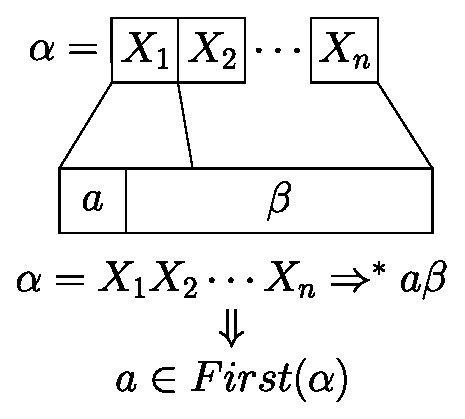
\includegraphics[width=0.4\textwidth]{obrazky-figures/first.eps}
    \caption{Ilustrace významu množiny \emph{First($\alpha$)} dle \cite{meduna2017sa-shora-dolu}.}
    \label{fig_mnozina_first}
\end{figure}

\begin{algorithm}[ht]
    \caption{Množina $First(\alpha)$}
    \label{alg_mnozina_first}
    \begin{algorithmic}[1]
        \Input{$G = (N, T, P, S)$}
        \Output{$First(\alpha)$ pro každé $\alpha \in (N \cup T)^*$}
        \NewLine
        \ForAll{$a \in T$}
            \State $First(a) \gets \{a\}$
        \EndFor
        \ForAll{$A \in N$}
            \State $First(A) \gets \emptyset$
        \EndFor
        \While{je možné měnit nějakou množinu $First(A)$}
            \If{$A \rightarrow X_1X_2\ldots X_{k-1}X_k\ldots X_n \in P$}
                \State $First(A) \gets First(A) \cup First(X_1)$
                \If{$Empty(X_1X_2\ldots X_{k-1}) = \{\varepsilon\}$}
                    \State $First(A) \gets First(A) \cup First(X_k)$ 
                \EndIf
            \EndIf
        \EndWhile
    \end{algorithmic}
\end{algorithm}
Je zřejmé, že řetězec derivovatelný z~terminálů $a$ musí určitě začínat terminálem $a$.
Ve druhém kroku algoritmu nastavíme $First(A)$ na prázdnou množinu, bude se měnit až v~dalších krocích.
Řetězec derivovatelný z~neterminálu $A$ pak může začínat:
\begin{enumerate}
    \item terminály z~množiny $First(\alpha_1)$, ať už se jedná o~terminál či neterminál,
    \item terminály z~množiny $First(\alpha_k)$, pokud řetězec neterminálů $X_1X_2\ldots X_{k-1}$ může být vymazán, respektive $Empty(X_1X_2\ldots X_{k-1}) = \varepsilon$.  
\end{enumerate}
Pro snadnější definici množiny $Follow(A)$ si uveďme algoritmus množiny $First(\alpha)$ pro neprázdné řetězce.
\begin{algorithm}
    \caption{Množina $First(\alpha_1\alpha_2\ldots\alpha_n)$}
    \label{alg_mnozina_first_vicn}
    \begin{algorithmic}[1]
        \Input{BKG $G = (N, T, P, S)$ a~$Empty(\alpha), First(\alpha)$ pro všechny symboly $\alpha \in N \cup T$}
        \Output{množiny $First(\alpha_1\alpha_2\ldots\alpha_n)$, kde ($\alpha_1\alpha_2\ldots \alpha_n) \in (N \cup T)^+$}
        \NewLine
        \State $First(\alpha_1\alpha_2\ldots \alpha_n) \gets First(\alpha_1)$
        \While{je možné měnit nějakou množinu $First(\alpha_1\alpha_2\ldots\alpha_{k-1}\alpha_k\ldots\alpha_n)$}
            \If{$Empty(\alpha_1\alpha_2\ldots\alpha_{k-1}) = \varepsilon$}
                \State $First(\alpha_1\alpha_2\ldots\alpha_n) \gets First(\alpha_1\alpha_2\ldots\alpha_n) \cup First(\alpha_k)$
            \EndIf
        \EndWhile
    \end{algorithmic}
\end{algorithm}

Další velmi podstatnou množinou, kterou syntaktický analyzátor potřebuje, je množina $Follow(A)$.
Ta určuje, jaké symboly se mohou vyskytovat za neterminálem $A$.
Nutnost této znalosti vyplývá z~možnosti přepsat neterminály, pro které platí $Empty(A) = \{\varepsilon\}$, na prázdný řetězec.
Kdyby analyzátor tuto množinu neměl k~dispozici, neměl by v těchto případech jak zjistit, zda je aktuální symbol na vstupu korektní nebo ne.
K~definici množin $Follow(A)$ se používá pomocný symbol \$, který reprezentuje konec vstupního řetězce.
\begin{definition}\label{def_mnozina_follow}
    Nechť $G = (N, T, P, S)$ je BKG.\\
    Pro všechny neterminály $A \in N$ definujeme množinu $Follow(A)$ jako
    \begin{align*}
        Follow(A) = \,&\{a: a \in T,\; S \Rightarrow^* \alpha Aa\beta,\; \alpha, \beta \in (N \cup T)^*\}\, \cup \\
                      &\{\$: S \Rightarrow^* \alpha A,\; \alpha \in (N \cup T)^*\}.
    \end{align*}
\end{definition}
\begin{algorithm}[h!]
    \caption{Množina $Follow(A)$}
    \label{alg_mnozina_follow}
    \begin{algorithmic}[1]
        \Input{BKG $G = (N, T, P, S)$}
        \Output{$Follow(A)$ pro každé $A \in N$}
        \NewLine
        \State $Follow(S) \gets \$$
        \While{je možné měnit nějakou množinu $Follow(A)$}
            \If{$A \rightarrow \alpha B\beta \in R$}
                \If{$\beta \neq \varepsilon$}
                    \State $Follow(B) \gets Follow(B) \cup First(\beta)$
                \EndIf
                \If{$Empty(\beta) = \{\varepsilon\}$}
                    \State $Follow(B) \gets Follow(B) \cup Follow(A)$
                \EndIf
            \EndIf
        \EndWhile 
    \end{algorithmic}
\end{algorithm}

Z~uvedené Definice \ref{def_mnozina_follow} a~Algoritmu \ref{alg_mnozina_follow} vyplývá, že v~množině $Follow(A)$ se mohou vyskytovat:
\begin{enumerate}
    \item terminální symboly vyskytující se za neterminálem $A$ v~libovolném zderivovaném řetězci,
    \item symbol ukončující vstupní řetězec, pokud za neterminálem $A$ již nebudou žádné další neterminály. 
\end{enumerate}

Množina $Follow(A)$ byla poslední množina, která byla třeba definovat, abychom mohli definovat množinu $Predict(A \rightarrow \alpha)$, ze které se poté může zkonstruovat \emph{LL tabulka}.
Množina $Predict(A \rightarrow \alpha)$ už je prakticky dobře použitelná pro syntaktickou analýzu\,--\,je to množina všech terminálů, které mohou být aktuálně nejlevěji vygenerovány, pokud pro libovolnou větnou formu použijeme pravidlo $A \rightarrow \alpha$.
\begin{definition}
    Nechť $G = (N, T, P, S)$ je BKG.\\
    Pro každé pravidlo $A \rightarrow \alpha \in P$ definujeme množinu $Predict(A \rightarrow \alpha)$ jako
    \begin{equation*}
        Predict(A \rightarrow \alpha) = First(\alpha) \cup Follow(A)
    \end{equation*}
    pokud $Empty(\alpha) = \{\varepsilon\}$,
    \begin{equation*}
        Predict(A \rightarrow \alpha) = First(\alpha)
    \end{equation*}
    pokud $Empty(\alpha) = \emptyset$.
\end{definition}
Prakticky díky této množině je syntaktický analyzátor schopen deterministicky vybrat pravidlo, které se aplikuje.
Mějme dvě pravidla, $p$ a~$q$, mezi kterými se analyzátor rozhoduje a~nechť na vstupu je terminál $a$.
Pokud $a \in Predict(p)$, pak se vybere pravidlo $p$, pokud $a \in Predict(q)$, pak se vybere pravidlo $q$.
Jak už bylo zmiňováno na začátku této kapitoly, všechny množiny $Predict(p)$ musí být navzájem disjunktní, jinak by výběr byl opět nedeterministický.
Tento koncept je aplikován v~\emph{LL(1) gramatikách}.

\subsection*{LL gramatiky}

Výše uvedené množiny pracují s~gramatikami, které se nazývají \emph{LL(1) gramatiky}.
Obecně gramatiky mohou být \emph{LL(k)}.
To jsou gramatiky, u~kterých stačí $k$ vstupních tokenů k~tomu, aby jejich analyzátor mohl deterministicky vybrat pravidlo pro aktuální neterminál.
Obecně platí, že LL(1) gramatiky jsou slabší (generují podmnožinu jazyků) než BKG \cite{medunaElementsOfCompDesign}.
LL(1) gramatika je definována následovně:
\begin{definition}
    Nechť $G = (N, T, P, S)$ je BKG.\\
    $G$ je \emph{LL(1) gramatikou}, pokud pro libovolná dvě pravidla $p, q \in P$ platí
    \begin{equation*}
        p \neq q \text{ a zároveň } Predict(p) \cap Predict(q) = \emptyset.
    \end{equation*}
\end{definition}
Jinými slovy neexistuje žádné $a \in T$ a~$A \in N$ takové, že $A \rightarrow \alpha, A \rightarrow \beta \in P$ a~zároveň $a \in First(\alpha)$ a~$a \in First(\beta)$.

\begin{convention}
    Tato práce se zabývá především LL(1) gramatikami.
    Pro zjednodušení, LL(1) gramatiky budou implicitně označovány jako \emph{LL gramatiky}.
    Bude-li se jednat o~LL($k$), bude to explicitně zapsáno.
\end{convention}

Některé bezkontextové gramatiky se dají převést na ekvivalentní LL gramatiky pomocí technik \emph{faktorizace} (vytýkání) a~\emph{odstranění levé rekurze}.

Myšlenka faktorizace je vytknutí stejné sekvence terminálů, která je společným prefixem několika pravých stran pravidel a~nahrazení zbývajícího řetězce za nový neterminál.
Z~nového neterminálu dále vznikají nová pravidla.
Například, mějme tato pravidla:
\begin{align*}
    A &\rightarrow a\alpha_1\\
    A &\rightarrow a\alpha_2\\
      &\vdotswithin{\rightarrow} \\
    A &\rightarrow a\alpha_n
\end{align*}
Terminál $a$ se může vytknout a~místo $\alpha_1, \alpha_2, \ldots, \alpha_n$ se vloží nový neterminál $B$, ze kterého se dále generují $\alpha_1, \alpha_2, \ldots, \alpha_n$.
\begin{align*}
    A &\rightarrow aB\\
    B &\rightarrow \alpha_1\\
    B &\rightarrow \alpha_2\\
      &\vdotswithin{\rightarrow}\\
    B &\rightarrow \alpha_n
\end{align*}

Levá rekurze je případ, kdy stejný neterminál, jako je na levé straně pravidla, je zároveň nejlevějším symbolem řetězce na pravé straně pravidla, například:
\begin{align*}
    A &\rightarrow A\alpha\\
    A &\rightarrow a
\end{align*}
Tato pravidla se dají přepsat do tvaru:
\begin{align*}
    A &\rightarrow aB\\
    B &\rightarrow \alpha B\\
    B &\rightarrow \varepsilon
\end{align*}
\todo{opet by to chtelo nejaky obrazky}

\subsection*{LL tabulka a její konstrukce}
\emph{LL tabulka} je abstrakcí k~množinám $Predict(p)$ jednotlivých pravidel LL gramatiky $G = (N, T, P, S)$.
Řádky tabulky jsou indexovány neterminály z~množiny $N$, sloupce potom terminály z~množiny $T \cup \{\$\}$.
Samotné položky tabulky jsou čísla pravidel, která byla přidělena funkcí mapující dvojici $(A, a),\; a \in T \cup \{\$\},\; A \in N$ na 
\begin{itemize}
    \item pravidlo, respektive symbol reprezentující konkrétní pravidlo,
    \item symbol vyjadřující neexistenci pravidla pro danou dvojici; v~tomto případě syntaktická analýza zahlašuje chybu.
\end{itemize}
Jinak řečeno, nechť $\alpha(A, a)$ reprezentuje políčko v~LL tabulce a~nechť $p: A \rightarrow X_1X_2\ldots X_n \in P$.
Pokud $a \in First(X_1)$, pak $\alpha(A, a) = p$, jinak nastává chyba.
Následující příklad převzat z~\cite{medunaElementsOfCompDesign}.
\begin{example}
    Nechť $G = (N, T, P, S)$ je LL gramatika a~nechť má sestavené množiny $Predict(p)$ pro každé $p \in P$.\\
    Pravidla a~jejich množiny $Predict$ nechť jsou definovány následovně: 
    \begin{table}[ht]
        \centering
        \begin{tabularx}{0.4\textwidth}{p{0.23\textwidth}p{0.17\textwidth}}
            \toprule
            Pravidlo $r \in R$ & $Predict(r)$ \\
            \midrule
            $E \rightarrow TA$      & $i, ($ \\
            $A \rightarrow \vee\; TA$ & $\vee$ \\
            $A \rightarrow \varepsilon $ & $), \$$ \\
            $T \rightarrow FB$ & $i, ($ \\
            $B \rightarrow \wedge\; FB$ & $\wedge$ \\
            $B \rightarrow \varepsilon$ & $\vee, )$ \\ 
            $T \rightarrow F$ & $i, ($ \\
            $T \rightarrow (E)$ & $($ \\
            $F \rightarrow i$ & $i$ \\
            \bottomrule
        \end{tabularx}
        \caption{Pravidla $G$ a jejich množiny $Predict$.}
        \label{tab_rules_predict}
    \end{table}
    
    Nechť symbol $\times$ reprezentuje prázdné políčko LL tabulky.
    LL tabulka pro pravidla a~jejich $Predict$ množiny z~tabulky \ref{tab_rules_predict}, zkonstruována podle výše popsané metody, vypadá takto:
    \begin{table}[h]
        \centering
        \begin{tabularx}{0.34\textwidth}{X|XXXXXX}
            \hline 
            $i$ & $i$ & $\vee$ & $\wedge$ & $($ & $)$ & $\$$ \\
            \hline
            $E$ & $1$ & $\times$ & $\times$ & $1$ & $\times$ & $\times$ \\
            $A$ & $\times$ & $2$ & $\times$ & $\times$ & $3$ & $3$ \\
            $T$ & $4$ & $\times$ & $\times$ & $4$ & $\times$ & $\times$ \\
            $B$ & $\times$ & $6$ & $5$ & $\times$ & $6$ & $6$ \\
            $F$ & $9$ & $\times$ & $\times$ & $8$ & $\times$ & $\times$ \\
            \hline
        \end{tabularx}
        \caption{LL tabulka pro pravidla z~tabulky \ref{tab_rules_predict}.}
        \label{tab_ll_table}
    \end{table}
\end{example}

\subsection*{Prediktivní syntaktická analýza}
\emph{Prediktivní syntaktická analýza} a~\emph{rekurzívní sestup} jsou dvě metody, pomocí kterých lze implementovat syntaktický analyzátor.
Jak je zmíněno na začátku této kapitoly, je potřeba nějakým způsobem provádět analýzu pomocí zásobníkového automatu.
Při použití prediktivní analýzy je nutné tento zásobník implementovat explicitně, rekurzívní sestup si zásobník tvoří v~pozadí automaticky díky volání funkcí pro každý neterminál.
Součástí této práce je implementace explicitního zásobníkového automatu, proto nebude rekurzívní sestup podrobně popsán; této metodě se detailně věnuje autor v~\cite{medunaElementsOfCompDesign}.

Výhodou implementace prediktivní analýzy s~LL tabulkou je jediná implementace algoritmu.
V~případě změny pravidel v~gramatice je nutné pouze změnit LL tabulku, odkud automat odebírá pravidla, která má použít.
Oproti tomu v~rekurzívním sestupu je nutné měnit celé funkce.
Algoritmus prediktivní syntaktické analýzy je popsán v~Algoritmu \ref{alg_prediktivni_sa}.
\begin{algorithm}[ht]
    \caption{Prediktivní syntaktická analýza založená na LL tabulce}
    \label{alg_prediktivni_sa}
    \begin{algorithmic}[1]
        \Input{LL tabulka pro $G = (N, T, P, S)$, řetězec $x \in T^*$}
        \Output{Levý rozbor pro $x$, pokud $x \in L(G)$, jinak chyba.}
        \NewLine
        \State \texttt{stack.push(\$)} \textbf{and} \texttt{stack.push(S)}
        \Repeat
            \State $X \gets$ \texttt{stack.top()}
            \State $a \gets$ aktuální token ze vstupního řetězce
            \Switch{$X$}
                \Case{\$}
                    \If{$a = \$$}
                        \State úspěch
                    \Else 
                        \State chyba
                    \EndIf
                \EndCase
                \Case{$X \in T$}
                    \If{$X = a$}
                        \State \texttt{stack.pop(X)}
                        \State $a \gets$ nový token ze vstupního řetězce
                    \Else
                        \State chyba
                    \EndIf
                \EndCase
                \Case{$X \in N$}
                    \If{$r: X \rightarrow \alpha \in LL\;table[X, a]$}
                        \State \texttt{stack.pop(X)}
                        \State \texttt{stack.top()} $\gets reversal(\alpha)$
                    \Else
                        \State chyba
                    \EndIf
                \EndCase
            \EndSwitch                
        \Until{úspěch \textbf{or} chyba}
    \end{algorithmic}
\end{algorithm}

\section{Syntaktická analýza zdola nahoru}\label{kap_sa_zdola_nahoru}
Syntaktická analýza zdola nahoru provádí konstrukci derivačního stromu zleva doprava a~zespodu nahoru, tudíž jde od listových uzlů (tokenů) směrem nahoru ke kořeni (výchozí neterminál) a~provádí nejpravější derivaci vstupního řetězce.
Každý krok této metody je reprezentován operacemi posunu (\emph{shift}) nebo redukce (\emph{reduce}).
Operace shift provádí vložení symbolu na zásobník a~redukce simuluje nejpravější derivační krok.
Během redukce analyzátor musí na zásobníku najít pravou stranu libovolného pravidla (nazývanou \emph{handle}), zredukovat jej a~výsledný neterminál vložit zpět na zásobník.

Pro tuto práci je důležitá pouze jedna z~metod analýzy zdola nahoru, a~to \emph{precedenční analýza výrazů}.
Existují další metody, jako je například \emph{LR syntaktická analýza}, ta ale není předmětem této práce, popsána bude pouze precedenční analýza.
LR analýza je podrobně popsána v~\cite{medunaElementsOfCompDesign}.

\subsection*{Precedenční analýza výrazů}
Precedenční analyzátor pracuje na základě $G = (N, T, P, S)$ pomocí \emph{precedenční tabulky}.
Precedenční tabulka je struktura se sloupci i~řádky tvořenými symboly z~množiny $T \cup \{\$\}$, kterými se tabulka v~praxi indexuje.
Každé pole precedenční tabulky má hodnotu jednoho ze symbolů množiny $\{<, >, =, \times, \text{\checkmark}\}$.

Analyzátor si na zásobník ukládá terminály i~neterminály a~navíc speciální znak $<$, který určuje počátek řetězce připravený na redukci.
Dno zásobníku pak reprezentuje symbol \$; zásobníková abeceda toho analyzátoru je tedy $T \cup \{<, \$\}$.

Než bude ukázán algoritmus pro precedenční analýzu, je třeba zadefinovat operace \emph{SHIFT} a~\emph{REDUCE}, se kterými analyzátor pracuje.
\begin{definition}
    Nechť $G = (N, T, P, S)$.\\
    Precedenční syntaktický analyzátor pracující na základě $G$ používá tyto operace pro práci se zásobníkem:
    \begin{itemize}
        \item $SHIFT(<)$ přesune řetězec $<a,\; a \in T$ na vrchol zásobníku a~přečte další symbol ze vstupu,
        \item $SHIFT(=)$ přesune vstupní symbol $a \in T$ na vrchol zásobníku a~přečte další symbol ze vstupu,
        \item $REDUCE(A \rightarrow \alpha)$, kde $A \in N,\; \alpha = a\beta,\; a \in T,\; \beta \in (N \cup T)^*$ nahradí řetězec $\alpha$ za $A$ na vrcholu zásobníku.
    \end{itemize}
\end{definition}
Funkcionalita precedenčního analyzátoru demonstrována na Algoritmu \ref{alg_precedencni_sa}.
Informace k tomuto algoritmu čerpány z~\cite{medunaElementsOfCompDesign,meduna2017sa-zdola-nahoru}, inspirace zápisu čerpána z~\cite{kunda2022}.
\begin{algorithm}[h]
    \caption{Precedenční syntaktický analyzátor}
    \label{alg_precedencni_sa}
    \begin{algorithmic}[1]
        \Input{Precedenční tabulka pro $G = (N, T, P, S)$, $x \in T^*$ ukončený symbolem \$}
        \Output{Pravý rozbor $x$, pokud $x \in L(G)$; jinak chyba}
        \NewLine
        \State \texttt{stack.push(\$)}
        \Repeat
            \Switch{Tabulka[\texttt{topmost\textunderscore token, input\textunderscore token}]}
                \Case{$=$}
                    \State $SHIFT(=)$
                \EndCase
                \Case{$<$}
                    \State $SHIFT(<)$
                \EndCase
                \Case{$>$}
                    \If{\texttt{stack.top()} = $<\alpha$ \textbf{and} $r: A \rightarrow \alpha \in R$}
                        \State $REDUCE(A \rightarrow \alpha)$
                    \Else
                        \State chyba \Comment{neexistuje pravidlo pro řetězec na zásobníku}
                    \EndIf
                \EndCase
                \Case{$\times$}
                    \State chyba \Comment{tabulka detekovala chybu}
                \EndCase
                \Case{\checkmark}
                    \State úspěch
                \EndCase
            \EndSwitch
        \Until{chyba \textbf{or} úspěch}
    \end{algorithmic}
\end{algorithm}

Jednotlivé kroky analýzy jsou určeny precedenční tabulkou, jejíž řádek je indexován nejvrchnějším (\emph{topmost}) terminálem na zásobníku a~sloupec je indexován vstupním terminálem, případně symbolem~\$.
Pokud je v~políčku tabulky symbol $=$ nebo $<$, pak analyzátor provede operaci $SHIFT$.
Je-li varianta $SHIFT(<)$, pak je nejdříve na zásobník vložen symbol $<$, a~to před první terminál, který se na zásobníku vyskytuje\,--\,pokud je na vrcholu zásobníku neterminál, přeskočí se.
Slouží k~rozpoznání řetězce, který má být v~rámci redukce na zásobníku nahrazen.
Poté se vloží na zásobník i~vstupní symbol a~přečte se nový ze vstupního řetězce.
Pokud je v~tabulce na políčku $>$, pak proběhne operace $REDUCE$, při které:
\begin{enumerate}
    \item najde na zásobníku řetězec $\alpha$, který má být zredukován (přepsán) řetězcem novým,
    \item určí pravidlo, u kterého se pravá strana rovná řetězci $\alpha$,
    \item nahradí řetězec $\alpha$ levou stranou určeného pravidla.
\end{enumerate}
Když tabulka vrátí symbol $\times$, nastává chyba. 
Při symbolu \checkmark analýza končí úspěšně.

Na následujícím příkladu z~\cite{medunaElementsOfCompDesign} je ukázán princip fungování Algoritmu \ref{alg_precedencni_sa}.
\begin{example}
    Nechť $G = (N, T, P, S)$ je BKG a~nechť množina $R$ obsahuje tato pravidla:
    \begin{align*}
        1: C &\rightarrow C \vee C \\
        2: C &\rightarrow C \wedge C \\
        3: C &\rightarrow (C) \\
        4: C &\rightarrow i
    \end{align*}
    A~předpokládejme precedenční tabulku s~těmito hodnotami:
    \begin{table}[h]
        \centering
        \begin{tabularx}{0.34\textwidth}{X|XXXXXX}
            \hline 
            & $\wedge$ & $\vee$ & $i$ & $($ & $)$ & \$ \\
            \hline
            $\wedge$ & $>$ & $>$ & $<$ & $<$ & $>$ & $>$ \\
            $\vee$ & $<$ & $>$ & $<$ & $<$ & $>$ & $>$ \\
            $i$ & $>$ & $>$ & $\times$ & $\times$ & $>$ & $>$ \\
            $($ & $<$ & $<$ & $<$ & $<$ & $=$ & $>$ \\
            $)$ & $>$ & $>$ & $\times$ & $\times$ & $>$ & $>$ \\
            \$ & $<$ & $<$ & $<$ & $<$ & $\times$ & \checkmark \\
            \hline 
        \end{tabularx}
        \caption{Precedenční tabulka pro pravidla $G$.}
    \end{table}

    Nechť vstupní řetězec je $i \wedge (i \vee i)\$$.
    \todo{obrazek dvou moznych derivacnich stromu}
    Analýza toho řetězce je znázorněna v~Tabulce \ref{tab_priklad_precedencni}.
    \begin{table}[h]
        \centering
        \begin{tabularx}{0.85\textwidth}{p{0.24\textwidth}rrp{0.27\textwidth}}
            \toprule
            \textbf{Zásobník} & \textbf{Precedence} & \textbf{Vstup} & \textbf{Akce} \\
            \midrule
            $\underline{\$}$                   & $[\$, i] \rightarrow \; <$                  & $\underline{i} \wedge (i \vee i)\$$ & $SHIFT(<)$ \\
            $\$<\underline{i}$                 & $[i, \wedge] \rightarrow \; >$              & $\underline{\wedge} (i \vee i)\$$   & $REDUCE(C \rightarrow i)$ \\
            $\underline{\$}C$                  & $[\$ ,\wedge] \rightarrow \; <$             & $\underline{\wedge} (i \vee i)\$$  & $SHIFT(<)$ \\
            $\$<C\underline{\wedge}$           & $[\wedge, (] \rightarrow \; <$              & $\underline{(}i \vee i)\$$          & $SHIFT(<)$ \\
            $\$<C\wedge<\underline{(} $        & $[(, i] \rightarrow \; < $                  & $\underline{i} \vee i) \$ $         & $SHIFT(<) $ \\
            $\$<C\wedge<(<\underline{i} $      & $[i, \vee] \rightarrow \; > $               & $\underline{\vee} i)\$ $            & $REDUCE(C \rightarrow i) $ \\
            $\$<C\wedge<\underline{(}C $       & $[(, \vee] \rightarrow \; < $               & $\underline{\vee} i)\$ $            & $SHIFT(<)$ \\
            $\$<C\wedge<(<C\underline{\vee}$   & $[\vee, i] \rightarrow \; <  $              & $\underline{i})\$ $                 & $SHIFT(<)$ \\
            $\$<C\wedge<(<C\vee<\underline{i}$ & $[i, )] \rightarrow \; > $                  & $\underline{)}\$ $                  & $REDUCE(C \rightarrow i)$ \\
            $\$<C\wedge<(<C\underline{\vee}C$  & $[\vee, )] \rightarrow \; > $               & $\underline{)}\$ $                  & $REDUCE(C \rightarrow C \vee C)$ \\
            $\$<C\wedge<\underline{(}C$        & $[(, )] \rightarrow \; = $                  & $\underline{)}\$ $                  & $SHIFT(=)$ \\
            $\$<C\wedge<(C\underline{)}$       & $[), \$] \rightarrow \; > $                 & $\underline{\$} $                   & $REDUCE(C \rightarrow (C))$ \\
            $\$<C\underline{\wedge} C$         & $[\wedge, \$] \rightarrow \; > $            & $\underline{\$} $                   & $REDUCE(C \rightarrow C \wedge C)$ \\
            $\underline{\$}C$                  & $[\$, \$] \rightarrow \; \text{\checkmark}$ & $\underline{\$} $                   & úspěch \\
            \bottomrule
        \end{tabularx}
        \caption{Demonstrace Algoritmu \ref{alg_precedencni_sa}.}
        \label{tab_priklad_precedencni}
    \end{table}
\end{example}    
\todo{obrazek derivacniho stromu}

\subsection*{Konstrukce precedenční tabulky}
Doposud nebylo zmíněno, co znamenají položky precedenční tabulky pro analýzu výrazů.
Znaménka $<$, a~$>$ se interpretují jako priorita operátotů.
Mějme dva operátory, například $\odot$ a~$\bigtriangleup$.
Pokud $\odot < \bigtriangleup$, pak $\bigtriangleup$ má vyšší prioritu, a~v~algoritmu to znamená, že pravá strana pravidla obsahující operátor $\bigtriangleup$ bude redukována dříve než pravá strana obsahující operátor $\odot$ a~naopak.
Pravidla pro tvorbu tabulky jsou pak následující \cite{medunaElementsOfCompDesign,meduna2017sa-zdola-nahoru}:
\begin{enumerate}
    \item Pokud operátor $\bigtriangleup$ má vyšší matematickou prioritu než operátor $\odot$, pak $\bigtriangleup > \odot$ a~$\odot < \bigtriangleup$.
    \item Pokud operátory $\bigtriangleup$ a~$\odot$ jsou stejné matematické priority a~levě asociativní, pak $\bigtriangleup < \odot$ a~$\odot < \bigtriangleup$.
    Pro pravě asociativní operátory platí $\bigtriangleup > \odot$ a~$\odot > \bigtriangleup$.
    \item Pokud $a \in T$ může předcházet operandu $i$, pak $a < i$.
    \item Pokud $a \in T$ může následovat za operandem $i$, pak $i > a$.
    \item Závorky:
    \begin{enumerate}
        \item Pro jeden pár závorek platí $(=)$.
        \item Pro $a \in T \setminus \{) ,\$\}$ platí $( < a$.
        \item Pro $a \in T \setminus\{(, \$\}$ platí $a > )$.
        \item Pokud $a \in T$ může předcházet $($, pak $a < ($. 
        \item Pokud $a \in T$ může následovat za $)$, pak $) > a$.
    \end{enumerate}
    \item Nechť $\odot$ je libovolný operátor.
    Pak platí $\$ < \odot$ a~$\odot > \$$.
    Dále platí $\$ \text{ \checkmark } \$$.
    \item Zbytek tabulky je vyplněn symbolem $\times$.
\end{enumerate}

Precedenční analýza nedokáže pracovat s~$\varepsilon$-pravidly a~pravidly se stejnou pravou stranou pro jiné neterminály.
V~praxi se tedy většinou používá výhradně pro analýzu výrazů.
Často se kombinuje s~analýzou shora dolů (ať už prediktivní analýzou či rekurzívním sestupem), kdy analýza shora dolů kontroluje vstupní řetězec mimo výrazy a~pro výrazy předává řízení analýze precedenční.

\chapter{Implementace syntaktického analyzátoru pro jazyk Koubp}\label{kap_implementace}

\section{Přijímaný jazyk}\label{kap_prijimany_jazyk}

Jazyk \emph{Koubp} je založený na jazyce IFJ22, který je podmnožinou jazyka PHP 8, jenž byl specifikován v~rámci zadání projektu do předmětu Formální jazyky a překladače v~akademickém roce 2022/2023.
V~této kapitole jsou popsány především syntaktické konstrukty jazyka Koubp a~není podrobně popsána sémantika příkazů, protože sémantická analýza není předmětem této práce.
\dotaz{je mozne citovat zadani projektu? pokud ano, jak se k nemu dostat?}

\subsection*{Obecné vlastnosti}
Jazyk Koubp je strukturovaný jazyk.
Podporuje deklaraci funkcí a~proměnných, které při deklaraci musí být explicitně definovány.
Hlavní tělo programu se skládá z~prolínání sekvence příkazů a~definic funkcí, přičemž definice funkcí nemohou být vnořené, ale mohou se vzájemně rekurzívně volat.
Vstupním bodem programu není funkce \texttt{main()}, jak lze nalézt například u~jazyka C \cite{ISO-C-Standard}, analýza probíhá od začátku souboru.
Není podporováno slučování souborů se zdrojovým kódem pomocí příkazů \texttt{import}, \texttt{include} a~podobných a~tím vytvoření jediného modulu, který by bylo možné zkompilovat.
Ve zdrojovém souboru a~uživatelem definovaných funkcích může být větvení, iterace a~další běžné konstrukce.
Veškeré proměnné jsou lokální, i~v~rámci hlavního těla programu.
Proměnné mají rozsah platnosti v~\emph{bloku kódu}, což je sekvence příkazů ve složených závorkách \texttt{\{\}}.
Tyto bloky kódu se mohou libovolně zanořovat.
V jazyce Koubp nejsou důležité \emph{bílé mezery (whitespaces)}.
Klíčová slova jazyka jsou
\begin{center}
    \texttt{if, while, for, return, elseif, else, function, int, float, string, bool}.
\end{center}

Identifikátory proměnných jsou posloupnosti alfanumerických znaků a~znak \texttt{\textunderscore}; identifikátor nesmí začínat číslicí.
Regulárním výrazem zapsáno jako:
\begin{center}
    \texttt{[a-zA-Z\textunderscore][a-zA-Z0-9\textunderscore]*}
\end{center}

Jazyk Koubp podporuje čtyři datové typy, a~to \texttt{int, float, bool, string}.
Jejich literály jsou definovány následovně:
\begin{itemize}
    \item Celočíselné literály jsou neprázdná posloupnost číslic, regulární výraz je
    \begin{center}
        \texttt{[0-9]+}
    \end{center} 
    \item Literály pro desetinná čísla, respektive čísla s~plovoucí desetinnou čárkou, jsou neprázdná posloupnost číslic následovaná tečkou, za kterou je další neprázdná posloupnost číslic.
    \begin{center}
        \texttt{[0-9]+.[0-9]+}
    \end{center}
    \item Literály typu \texttt{bool} jsou \texttt{true} a~\texttt{false}.
    \item Řetězcové literály jsou posloupností (i~prázdnou) znaků uzavřenou v~uvozovkách.
    Pro zapsání speciálních znaků je možnost použít \emph{escape sekvence}, které začínají zpětným lomítkem.
    \begin{center}
        \texttt{\textbackslash"(\textbackslash\textbackslash.|[\^{}\textbackslash\textbackslash"])*\textbackslash"}
    \end{center}
\end{itemize}

Jsou také podporovány řádkové a~blokové komentáře.
Řádkový komentář je sekvence znaků počínající dvojitým lomítkem \texttt{//}, končí na konci aktuálního řádku.
Blokový komentář může být na více řádků počínaje znaky \texttt{/*}, konče znaky \texttt{*/}.

\subsection*{Deklarace a definice funkcí}
Jak bylo zmíněno v~úvodu této kapitoly, deklarované funkce musí být rovnou definovány.
Jazyk Koubp nepodporuje \emph{přetěžování (overloading)}\footnote{Pro C++ například \href{https://learn.microsoft.com/en-us/cpp/cpp/function-overloading?view=msvc-170}{https://learn.microsoft.com/en-us/cpp/cpp/function-overloading?view=msvc-170}. V~ostatních kompilátorech, jako \texttt{gcc}/\texttt{g++} nebo \texttt{clang}/\texttt{clang++} budou principy minimálně velmi podobné. } funkcí.
Definice funkce se skládá z~hlavičky za klíčovým slovem \texttt{function} a~těla funkce.
V~hlavičce se definuje název funkce, návratový typ a~počet parametrů a~jejich datové typy.
Schematicky vypadá následovně:
\begin{center}
    \texttt{function <jméno> ( <seznam parametrů> ) : <datový typ> \{ <tělo funkce> \}}
\end{center}
Dvojtečka před datovým typem musí být uvedena vždy, a~to i~v~případě, že funkce nemá návratovou hodnotu (takzvaně \texttt{void} funkce).
V~tomto případě za dvojtečkou ihned následuje levá složená závorka \texttt{\{}.
Parametry funkce jsou oddělené čárkami a~jejich struktura je:
\begin{center}
     \texttt{<datový typ>} \texttt{<jméno proměnné>}
\end{center}
Tělo funkce je pak neprázdná sekvence příkazů.
Příklad definice funkce je:
\begin{lstlisting}[language=Koubp]
    function factorial(int number): int {
        if (number < 0) {
            return -1;
        }
        elseif (number <= 1) {
            return 1;
        }

        return number * factorial(number - 1);
    }
\end{lstlisting}

\subsection*{Příkazy}
Jazyk Koubp podoruje obvyklé příkazy a~konstrukce jiných programovacích jazyků.
\begin{itemize}
    \item \emph{Přiřazení}\,--\,stejně, jako u~definic funkcí, deklarace není možná.
    Hodnota se může přiřadit do již definované proměnné nebo při vytvoření nové proměnné, která předtím definovaná nebyla.
    \begin{align*}
        \text{\texttt{<datový typ> <jméno proměnné> }} &\text{\texttt{= <hodnota>}} \\
        \text{\texttt{<jméno proměnné> }} &\text{\texttt{= <hodnota>}}        
    \end{align*}
    \item \emph{Větvení}\,--\,podmíněný příkaz podporuje klíčová slova \texttt{if}, \texttt{elseif}, \texttt{else}.
    Ačkoliv je možnost používat přímo klíčové slovo \texttt{elseif}, jazyk Koubp podporuje i~sekvenci \texttt{else if}, jejichž sémantický rozdíl je patrně vidět na obrázcích \ref{fig_ast_elseif} a~\ref{fig_ast_else_if}.
    Syntaxe je následující:
    \begin{lstlisting}[language=Koubp]
        if (vyraz) {
            sekvence_prikazu
        }
        elseif (vyraz) {
            sekvence_prikazu
        }
        else {
            sekvence_prikazu
        }
    \end{lstlisting}
    Je podporováno psát sekvence příkazů i~bez složených závorek \texttt{\{\}}.
    V tom případě se ke konstrukci vztahuje pouze první příkaz, který se za konstrukcí vyskytuje, podobně jako v~jazyce C \cite{ISO-C-Standard}.
    Tohle pravidlo platí i~pro příkazy nebo sekvence příkazů v~cyklech. 
    \begin{lstlisting}[language=Koubp]
        if (vyraz) 
            prikaz;
        elseif (vyraz)
            prikaz;
        else
            prikaz;
    \end{lstlisting}
    \begin{figure}[ht]
        \centering
        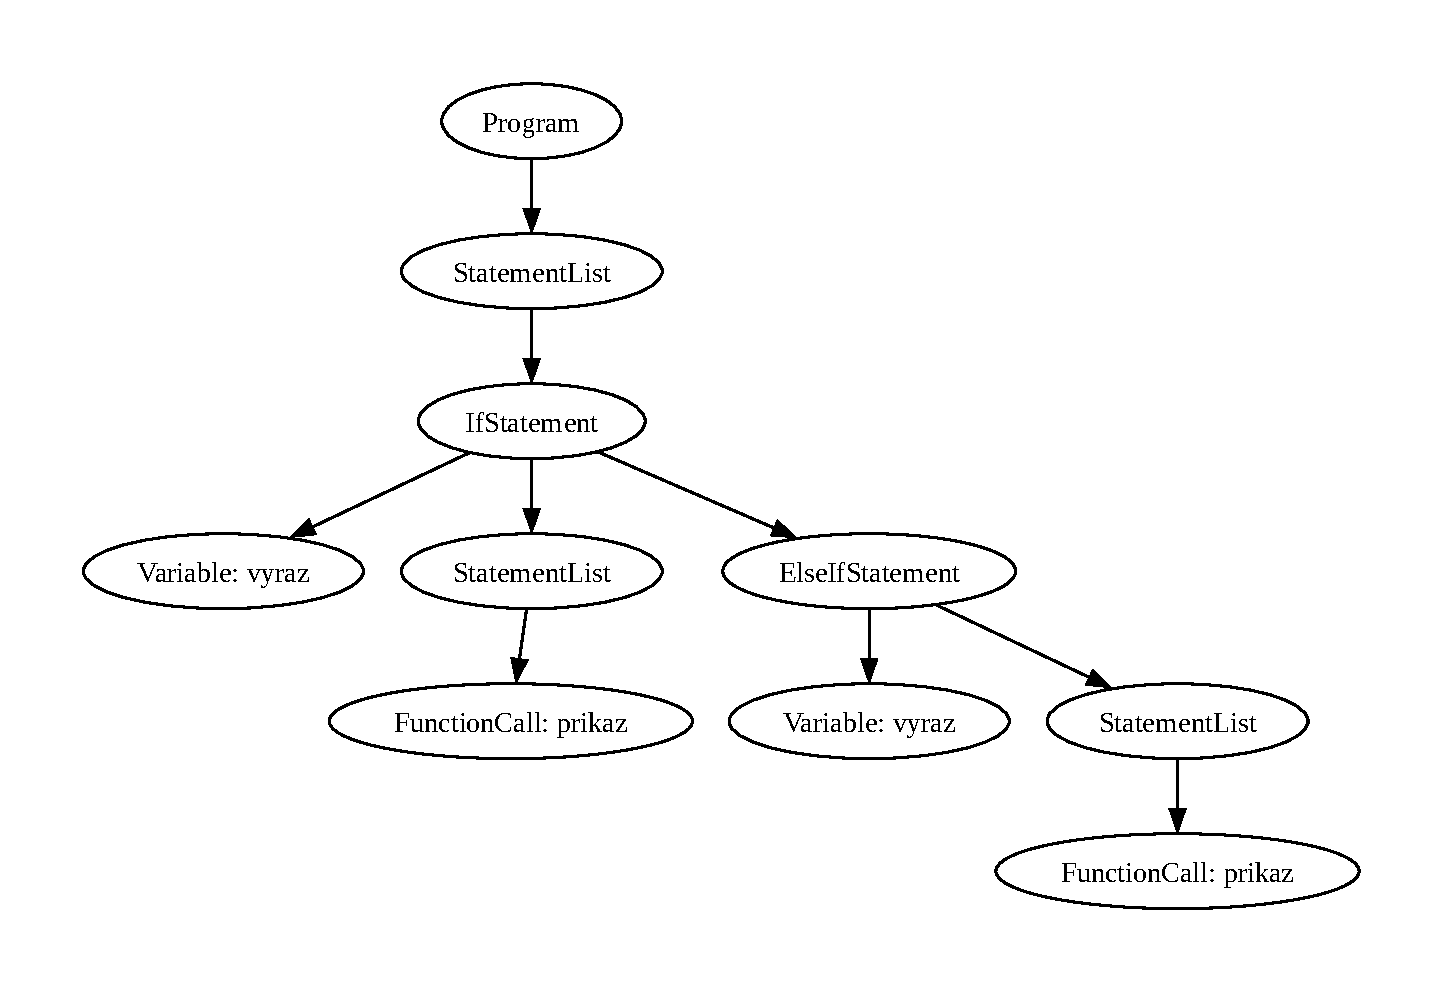
\includegraphics[width=0.8\textwidth]{obrazky-figures/ast_if_elseif.pdf}
        \caption{Programem vygenerovaný AST pro konstrukci \texttt{if-elseif}}
        \label{fig_ast_elseif}
    \end{figure}
    \begin{figure}[ht]
        \centering
        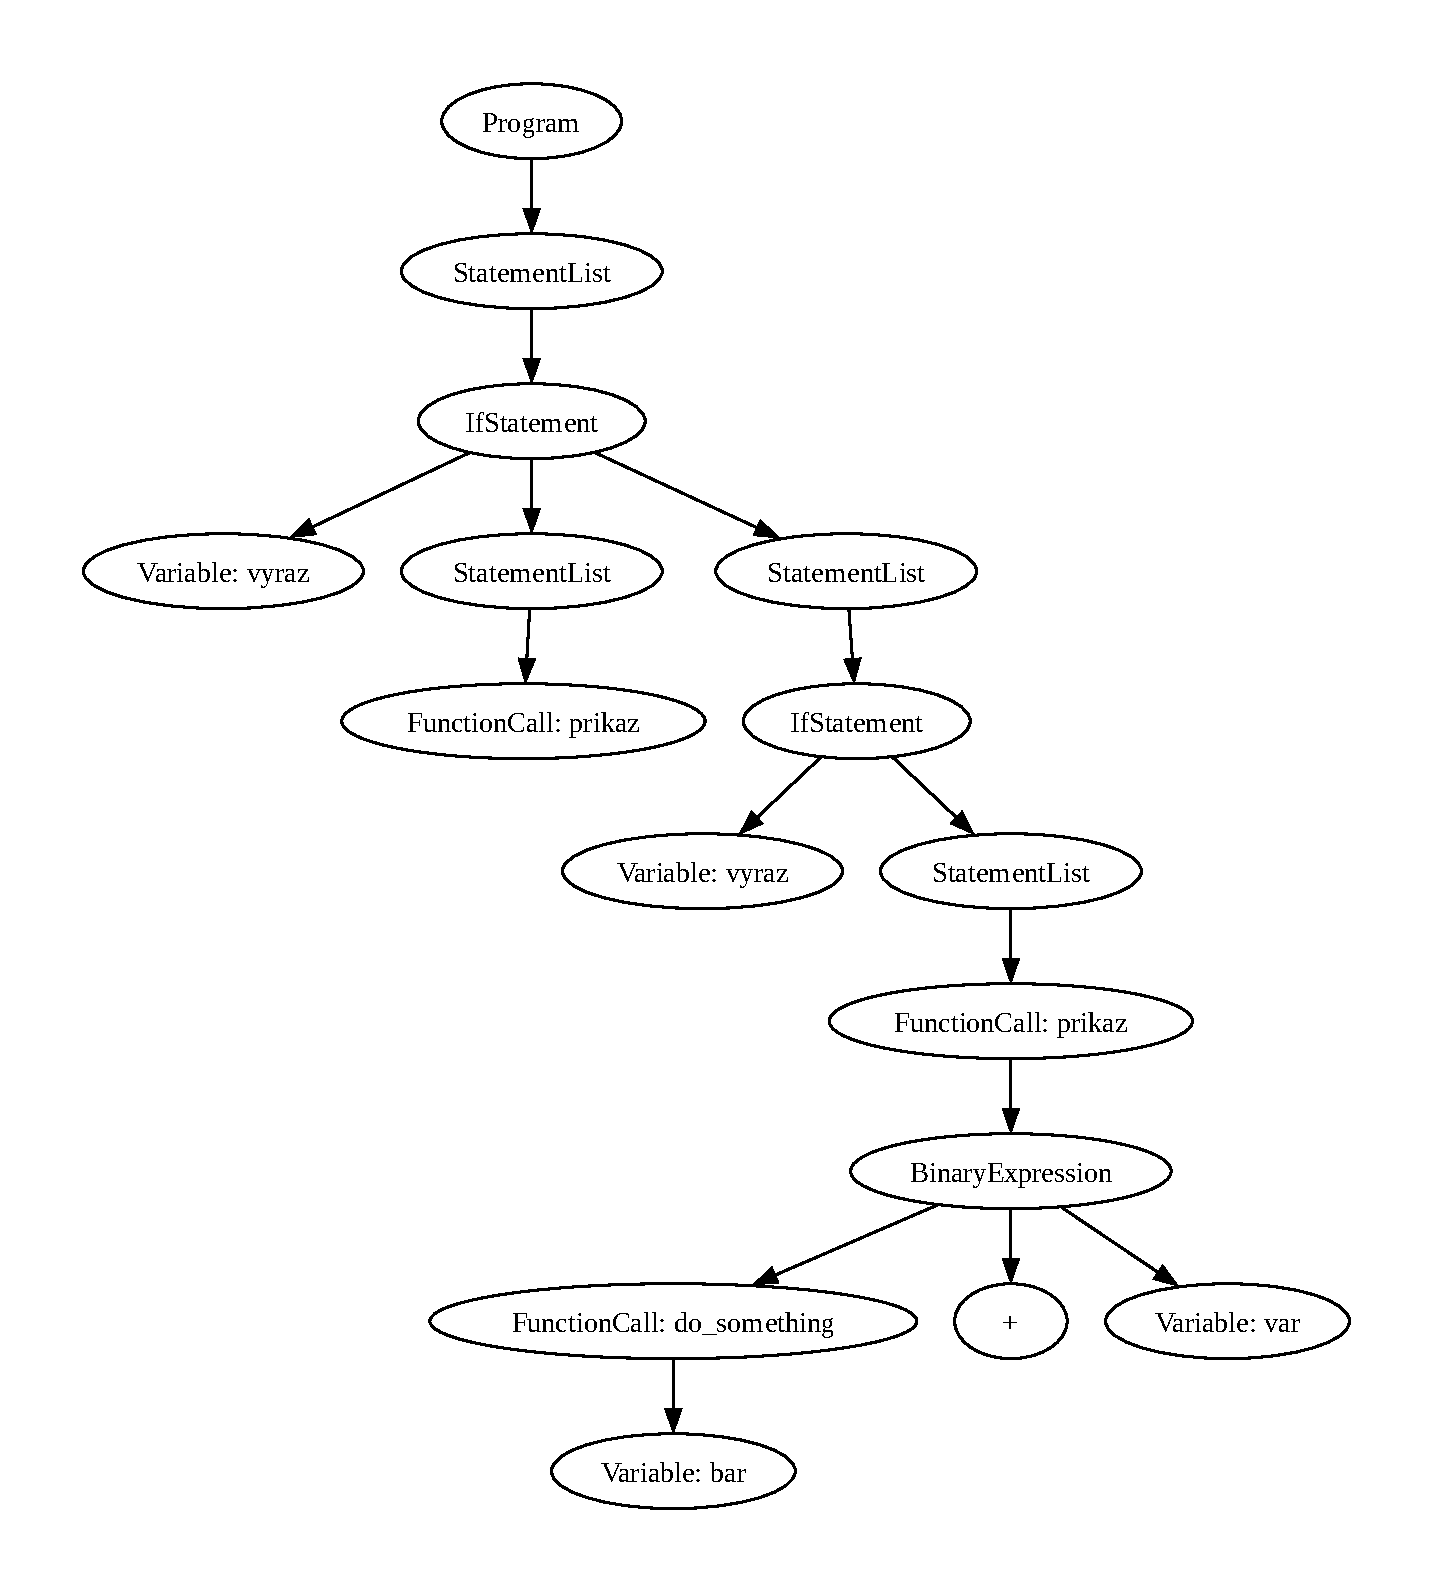
\includegraphics[width=0.8\textwidth]{obrazky-figures/ast_if_else_if.pdf}
        \caption{Programem vygenerovaný AST pro konstrukci \texttt{if-else if}}
        \label{fig_ast_else_if}
    \end{figure}
    \item \emph{Cyklus while}\,--\,Vykonává se sekvence příkazů (nebo příkaz) tak dlouho, dokud \emph{výraz} není vyhodnocen jako pravda.
    \begin{lstlisting}[language=Koubp]
        while (vyraz) {
            sekvence_prikazu
        }

        while (vyraz)
            prikaz;
    \end{lstlisting}
    \item \emph{Cyklus for} se skládá z~hlavičky a~těla.
    Hlavička se skládá ze tří částí\,--\,inicializace a~dva výrazy, všechny jsou odděleny středníkem.
    Inicializace může být výraz, deklarace nebo přiřazení.
    \begin{lstlisting}[language=Koubp]
        for (inicializace; vyraz; vyraz) {
            sekvence_prikazu
        }

        for (inicializace; vyraz; vyraz) 
            prikaz;
    \end{lstlisting}
    \item \emph{Příkaz return}\,--\,začíná klíčovým slovem \texttt{return} a~následuje volitelný výraz.
    Vrátí hodnotu výrazu z~volané funkce nebo spuštěného programu.
    \begin{lstlisting}[language=Koubp]
        return vyraz;
        return;
    \end{lstlisting}
\end{itemize}

\subsection*{Výrazy}
Výrazy jazyka Koubp jsou tvořeny operátory, operandy a~závorkami.
Mezi operandy se řadí proměnné, konstanty (literály) a~volání funkcí.

\begin{itemize}
    \item Operátory jsou unární (\texttt{! -}) a~binární, které se dále dělí na
    \begin{itemize}[label=$\circ$]
        \item aritmetické \texttt{. + - * /},
        \item logické \texttt{\&\& ||},
        \item relační \texttt{== != > < >= <=},
        \item přiřazení \texttt{=}.
    \end{itemize}
    Unární mínus je v~implementaci reprezentováno jiným tokenem než binární mínus.
    Na přiřazení se v~jazyce Koubp hledí jako na operátor s~nejmenší prioritou.
    Proto například výraz
    \begin{center}
        \texttt{variable = 1 + 2 + 3 = retezec1.retezec2;}
    \end{center}
    je syntakticky v~pořádku.
    O~dodatečnou kontrolu správnosti tohoto výrazu se musí postarat sémantická analýza. 
    \item Tabulka \ref{tab_priorita_operatoru} ilustruje prioritu operátorů sestupně a~jejich asociativitu.
    Asociativita udává, v~jakém pořadí se vyhodnotí operátory se stejnou prioritou.
    Například, mějme výraz
    \begin{center}
        1 + 2 + 3.
    \end{center}
    Pokud operátor \texttt{+} je levě asociativní, pak je výraz vyhodnocen jako
    \begin{center}
        (1 + 2) + 3,
    \end{center}
    v~opačném případě jako
    \begin{center}
        1 + (2 + 3).
    \end{center}
    Asociativita je důležitá především u~operátorů, které nejsou komutativní, jako například operátor dělení \texttt{/}.
    Nicméně se musí definovat pro všechny operátory, aby precedenční analyzátor věděl, který z~výrazů má vyhodnotit dříve.
    Implementačně to znamená, že výrazy s~operátory s~vyšší prioritou budou vyhodnoceny dříve než operátory s~nižší prioritou.
    \begin{table}[ht]
        \centering
        \begin{tabularx}{0.7\textwidth}{p{0.15\textwidth}p{0.3\textwidth}X}
            \toprule
            \textbf{Pořadí} & \textbf{Seznam operátorů} & \textbf{Asociativita} \\
            \midrule
            1) & \texttt{! -} & levá \\
            2) & \texttt{* /} & levá \\
            3) & \texttt{+ - .} & levá \\
            4) & \texttt{== != > < >= <=} & levá \\
            5) & \texttt{\&\& ||} & levá \\
            \bottomrule
        \end{tabularx}
        \caption{Priorita operátorů a jejich asociativita.}
        \label{tab_priorita_operatoru}
    \end{table}
    \item Volání funkce je bráno jako operand, který se může ve výrazech běžně používat.
    Dále má jako argumenty výrazy oddělené čárkami, tudíž se mohou libovolně zanořovat.
    Následující příklad je syntakticky správně v~jazyce Koubp.
    \begin{lstlisting}[language=Koubp]
        int p = foo(s1."bar\n", 8*7) + !convert_bool(readline());
    \end{lstlisting}
\end{itemize}

\subsection*{Vestavěné funkce}
Jazyk Koubp má několik vestavěných funkcí, které se ve zdrojovém kódu mohou použít bez jejich předchozí definice.
Dělí se na vstupně-výstupní funkce, funkce pro typovou konverzi a~funkce pro práci s~řetězci.

Vstupně-výstupní funkce pro práci se standardním vstupem/výstupem jsou:
\begin{itemize}
    \item \texttt{function print(string vyraz1, string vyraz2, \ldots)},
    \item \texttt{function readline(): string}.
\end{itemize}
Funkce \texttt{print()} na standardní výstup vypíše výrazy postupně zleva doprava bez oddělovačů.
Pro zapsání jiných typů než řetězce je možné použít funkce pro typovou konverzi, případně znak \texttt{\$} uvnitř řetězce pro vepsání hodnoty proměnné do řetězce.
Například v~následujícím příkladu
\begin{lstlisting}[language=Koubp]
    float cislo = 42.37;
    print("$cislo\n");
    print(convert_string(cislo)."\n");
\end{lstlisting}
se v~obou případech vypíše na standardní výstup stejný řetězec.
Pro vypsání znaku \texttt{\$} musí být použita escape sekvence, tudíž \texttt{\textbackslash\$}.
Pro konstantní hodnoty funguje pouze varianta s~funkcí \texttt{convert\textunderscore string()}.
Funkce \texttt{readline()} přečte sekvenci znaků ukončenou \texttt{\textbackslash n} ze standardního vstupu a~vrátí ji jako řetězec.

Pro práci se soubory jsou funkce
\begin{itemize}
    \item \texttt{function file\textunderscore open(string filename): int},
    \item \texttt{function file\textunderscore write(string filename, string buffer)},
    \item \texttt{function file\textunderscore readline(string filename): string},
    \item \texttt{function file\textunderscore close(string filename): int}.
\end{itemize}
Sémantika je očekáváná.
Funkce \texttt{file\textunderscore open()} otevře soubor specifikovaný v~parametru \texttt{filename} pro čtení nebo zápis a~vrací návratový kód pomocí kterého se může identifikovat chyba.
\texttt{file\textunderscore write()} zapíše do souboru \texttt{filename} řetězec v~parametru \texttt{buffer}.
Dále funkce \texttt{file\textunderscore readline()} přečte jeden řádek ze souboru, případně vrací prázdný řetězec a~funkce \texttt{file\textunderscore close()} zavře soubor \texttt{filename} pro čtení i~zápis, vrací návratový kód pro detekci chyby.

Typové konverze jsou uskutečněny funkcemi
\begin{itemize}
    \item \texttt{function convert\textunderscore int(term): int},
    \item \texttt{function convert\textunderscore string(term): string},
    \item \texttt{function convert\textunderscore float(term): float},
    \item \texttt{function convert\textunderscore bool(term): bool},
\end{itemize}
a~jsou to jediné vestavěné funkce, které pracují s~operandem libovolného datového typu.
Například:
\begin{lstlisting}[language=Koubp]
    int cislo = convert_int(readline());
    bool hodnota = convert_bool(cislo);
    print(convert_string(hodnota)); // Vypise "true" nebo "false" na stdin
\end{lstlisting}

Poslední vestavěné funkce jsou takové, které pracují s~řetězci.
Jsou to funkce
\begin{itemize}
    \item \texttt{function strlen(string s): int} a 
    \item \texttt{function substring(string s, int i, int j): string}.
\end{itemize}
Funkce \texttt{strlen()} vrací délku řetězce, který je dán jako parametr a~\texttt{substring()} vrátí podřetězec řetězce \texttt{s} od indexu \texttt{i} po index \texttt{j}.

\section{Gramatický systém definujíci syntax jazyka Koubp}
Gramatický systém popisující syntax jazyka Koubp je CD gramatický systém.
Formálně zapsáno, je to devítice $\Gamma = (N, T, S, P_1, P_2, P_3, P_4, P_6, P_6)$, kde:
\begin{align*}
    N & = 
        \begin{aligned}[t]
          \{&\texttt{PROGRAM}, \texttt{ STATEMENT\_LIST}, \texttt{ STATEMENT}, \texttt{ IF2}, \texttt{ DECLOREXP}, \texttt{ RETURNEXP},\\
            &\texttt{FUNCDEF}, \texttt{ PARAMS}, \texttt{ PARAMS2}, \texttt{ EXPRESSION}, \texttt{ ARGS}, \texttt{ ARGS2}, \texttt{ CODEBLOCK},\\
            &\texttt{STATEMENTS}, \texttt{ VOLTYPE}, \texttt{ TYPE}\}
        \end{aligned}\\
    T & = 
        \begin{aligned}[t]
          \{&\texttt{if}, \texttt{ elseif}, \texttt{ else}, \texttt{ while}, \texttt{ for}, \texttt{ return}, \texttt{ function}, \texttt{ int}, \texttt{ float},\\
            &\texttt{string}, \texttt{ bool}, \texttt{ variable}, \texttt{ constant}, \texttt{ functionName}, \texttt{ +}, \texttt{ -}, \texttt{ *}, \texttt{ /},\\
            &\texttt{.}, \texttt{ \&\&}, \texttt{ ||}, \texttt{ ==}, \texttt{ !=}, \texttt{ >}, \texttt{ <}, \texttt{ >=}, \texttt{ <=}, \texttt{ :}, \texttt{ ,}, \texttt{ (}, \texttt{ )}, \texttt{ \{} \texttt{ \}}\}
        \end{aligned}\\
    S & = \texttt{PROGRAM}
\end{align*}



Komponenty systému jsou navrhnuty tak, aby každá z~nich tvořila ucelenou část jazyka Koubp.
První komponenta popisuje strukturu programu\,--\,sekvence příkazů a~definic funkcí.
\begin{equation*}
    P_1 = \{ 
        \begin{aligned}[t] 
            &\texttt{PROGRAM \textrightarrow{} STATEMENT STATEMENT\textunderscore LIST},\\
            &\texttt{PROGRAM \textrightarrow{} FUNCDEF STATEMENT\textunderscore LIST},\\
            &\texttt{STATEMENT\textunderscore LIST \textrightarrow{} STATEMENT STATEMENT\textunderscore LIST},\\
            &\texttt{STATEMENT\textunderscore LIST \textrightarrow{} FUNCDEF STATEMENT\textunderscore LIST},\\
            &\texttt{STATEMENT\textunderscore LIST \textrightarrow{} }\varepsilon\}
        \end{aligned}
\end{equation*}

Druhá komponenta obsahuje seznam příkazů a~běžných konstrukcí doplněné o~jejich pomocné neterminály.
\begin{equation*}
    P_2 = \{ 
        \begin{aligned}[t] 
            &\texttt{STATEMENT \textrightarrow{} } \texttt{if ( EXPRESSION ) CODEBLOCK IF2},\\
            &\texttt{STATEMENT \textrightarrow{} } \texttt{while ( EXPRESSION ) CODEBLOCK},\\
            &\texttt{STATEMENT \textrightarrow{} } \texttt{for ( DECLOREXP; EXPRESSION; EXPRESSION ) CODEBLOCK},\\
            &\texttt{STATEMENT \textrightarrow{} } \texttt{DECLOREXP;},\\
            &\texttt{STATEMENT \textrightarrow{} } \texttt{CODEBLOCK},\\
            &\texttt{STATEMENT \textrightarrow{} } \texttt{return RETURNEXP;},\\
            &\texttt{STATEMENT \textrightarrow{} } \texttt{;},\\
            &\texttt{IF2 \textrightarrow{} } \texttt{elseif ( EXPRESSION ) CODEBLOCK IF2},\\
            &\texttt{IF2 \textrightarrow{} } \texttt{else CODEBLOCK},\\
            &\texttt{IF2 \textrightarrow{} } \varepsilon,\\
            &\texttt{DECLOREXP \textrightarrow{} } \texttt{TYPE variable = EXPRESSION},\\
            &\texttt{DECLOREXP \textrightarrow{} } \texttt{EXPRESSION},\\
            &\texttt{RETURNEXP \textrightarrow{} } \texttt{EXPRESSION},\\
            &\texttt{RETURNEXP \textrightarrow{} } \varepsilon\} 
        \end{aligned}
\end{equation*}


Třetí komponenta zahrnuje definici funkce a~pomocné neterminály.
\begin{equation*}
    P_3 = \{ 
        \begin{aligned}[t] 
            &\texttt{FUNCDEF \textrightarrow{} } \texttt{function functionName ( PARAMS ) : VOLTYPE \{ STATEMENTS \}},\\
            &\texttt{PARAMS \textrightarrow{} } \texttt{EXPRESSION PARAMS2}, \\
            &\texttt{PARAMS \textrightarrow{} } \varepsilon,\\
            &\texttt{PARAMS2 \textrightarrow{} } \texttt{, EXPRESSION PARAMS2},\\
            &\texttt{PARAMS2 \textrightarrow{} } \varepsilon \}
        \end{aligned}
\end{equation*}

Čtvrtá komponenta popisuje veškerou práci s~výrazy a~obsahuje pomocné neterminály pro volání funkcí.
Nechť symboly $\lfloor$ a~$\rceil$ ohraničují možnosti terminálů, které se v~daném pravidle mohou vyskytovat.
\begin{equation*}
    P_4 = \{ 
        \begin{aligned}[t] 
            &\texttt{EXPRESSION \textrightarrow{} } \texttt{EXPRESSION } \lfloor \texttt{+ - * / . \&\& || == != > < >= <= =}\rceil \texttt{ EXPRESSION},\\
            &\texttt{EXPRESSION \textrightarrow{} } \lfloor \texttt{! -} \rceil \texttt{ EXPRESSION}, \\
            &\texttt{EXPRESSION \textrightarrow{} } \texttt{variable},\\
            &\texttt{EXPRESSION \textrightarrow{} } \texttt{constant},\\
            &\texttt{EXPRESSION \textrightarrow{} } \texttt{functionName},\\
            &\texttt{EXPRESSION \textrightarrow{} } \texttt{( EXPRESSION )} \}
        \end{aligned}
\end{equation*}

Pátá komponenta pojednává o~bloku kódu, který byl vysvětlen v~úvodu Kapitoly \ref{kap_prijimany_jazyk}.
Důvod pro použití samostatné komponenty pro tuto konstrukci, a~ne znovupoužití neterminálu \texttt{STATEMENT\textunderscore LIST}, je explicitní zakázání zanořování definic funkcí.
V~této konstrukci se tedy mohou vyskytovat libovolné příkazy a~jejich sekvence, nesmí se tam objevit definice funkce. 
\begin{equation*}
    P_5 = \{ 
        \begin{aligned}[t] 
            &\texttt{CODEBLOCK \textrightarrow{} } \texttt{\{ STATEMENTS \}},\\
            &\texttt{CODEBLOCK \textrightarrow{} } \texttt{STATEMENT}, \\
            &\texttt{STATEMENTS \textrightarrow{} } \texttt{STATEMENT STATEMENTS},\\
            &\texttt{STATEMENTS \textrightarrow{} } \varepsilon \}
        \end{aligned}
\end{equation*}

Šestá komponenta obsahuje pouze neterminály související s~datovými typy.
\begin{equation*}
    P_6 = \{ 
        \begin{aligned}[t] 
            &\texttt{VOLTYPE \textrightarrow{} } \texttt{TYPE},\\
            &\texttt{VOLTYPE \textrightarrow{} } \varepsilon, \\
            &\texttt{TYPE \textrightarrow{} } \texttt{int},\\
            &\texttt{TYPE \textrightarrow{} } \texttt{float},\\
            &\texttt{TYPE \textrightarrow{} } \texttt{string},\\
            &\texttt{TYPE \textrightarrow{} } \texttt{bool} \}
        \end{aligned}
\end{equation*}

Všimněme si, že mezi neterminály \texttt{STATEMENT} a~\texttt{CODEBLOCK} teoreticky může nastat situace, kdy se tyto dva neterminály budou vzájemně derivovat donekonečna, přičemž oba budou čekat na jinou derivaci druhého a~nastane \emph{deadlock}.
Tato situace je vyřešená implementačně\,--\,neterminál \texttt{STATEMENT} bude derivovat neterminál \texttt{CODEBLOCK} jen a~pouze tehdy, bude-li na vstupu terminál \texttt{\{}.

\subsection*{Indexace neterminálů a LL tabulka}
Každému neterminálu z~množiny $N$ v~$\Gamma$ je přiřazen index, který odkazuje na různé komponenty $P_i \in \Gamma,\; i \in \{1, \ldots, 6\}$.
Každý neterminál má pravidla pro expanzi pouze v~jedné komponentě, díky čemuž je možné deterministicky zvolit komponentu, které se bude předávat řízení syntaktické analýzy.
Pomocí vstupního terminálu se poté v~komponentě zvolí pravidlo, které se použije pro expanzi.
Tato indexace lze matematicky popsat zobrazením z~množiny neterminálů do podmnožiny přirozených čísel, které korespondují s~indexy komponent v~konkrétním gramatickém systému.
V~tomto případě se jedná o~zobrazení
\begin{equation*}
    N \rightarrow \{i: P_i \in \Gamma\}
\end{equation*}
které je definováno v~Tabulce \ref{tab_zobrazeni_indexy}.
\begin{table}[ht]
    \centering
    \begin{tabularx}{0.5\textwidth}{Xc}
        \toprule
        \textbf{Neterminál} & \textbf{Index komponenty}\\
        \midrule
        \texttt{PROGRAM} & 1\\
        \texttt{STATEMENT\textunderscore LIST} & 1\\
        \texttt{STATEMENT} & 2\\
        \texttt{IF2} & 2\\
        \texttt{DECLOREXP} & 2\\
        \texttt{RETURNEXP} & 2\\
        \texttt{FUNCDEF} & 3\\
        \texttt{PARAMS} & 3\\
        \texttt{PARAMS2} & 3\\
        \texttt{EXPRESSION} & 4\\
        \texttt{ARGS} & 4\\
        \texttt{ARGS2} & 4\\
        \texttt{CODEBLOCK} & 5\\
        \texttt{STATEMENTS} & 5\\
        \texttt{VOLTYPE} & 6\\
        \texttt{TYPE} & 6\\
        \bottomrule
    \end{tabularx}
    \caption{Zobrazovací funkce neterminálů na indexy komponent.}
    \label{tab_zobrazeni_indexy}
\end{table}

LL tabulka syntaktického analyzátoru obsahuje kromě obvyklých čísel pravidel uspořádané dvojice \emph{(číslo komponenty, číslo pravidla)}.
Samotná tabulka je sestavena pomocí množin \emph{Empty($\alpha$)}, \emph{First($\alpha$)}, \emph{Follow(A)} a~\emph{Predict($A \rightarrow \alpha$)}.
První tři množiny se vytvoří standardním způsobem pro každý terminál a~neterminál.
Množina \emph{Predict($A \rightarrow \alpha$)} se sestavuje pro každé pravidlo, stejně jako u~LL gramatik, reprezentované uspořádanou dvojicí.
Prediktivní množiny a~LL tabulka pro GS $\Gamma$ popisující jazyk Koubp jsou v~příloze. \todo{ref priloha, vlozeni prilohy}

\section{Návrh řešení syntaktického analyzátoru}\label{kap_reseni_sa}
Implementace syntaktické analýzy je silně objektově orientována, veškeré datové struktury jsou reprezentovány třídami.
Třídy reprezentující neterminály a~terminály mají společnou nadtřídu, díky čemuž je možné je ukládat do jednoho zásobníku za použití polymorfismu.
Jednu nadtřídu mají také gramatiky, jednotlivé instance jsou poté konstruovány pomocí tovární metody.
Analyzátory jsou také reprezentovány třídami, společnou nadtřídu ale nemají.

\subsection*{Práce s~komponentami}
Všechny komponenty jsou využívány pouze prediktivním analyzátorem, mimo čtvrtou.
Ačkoliv téma čtvrté komponenty je analýza výrazů, je využívána jak precedenčním, tak prediktivním analyzátorem.
Důvod je zvolený postup prediktivní analýzy volání funkcí\,--\,o~samotné výrazy bez volání funkcí, tedy pouze výrazy s~konstantami a~proměnnými, se postará analýza precedenční, správnou posloupnost terminálů pro volání funkcí kontroluje analýza prediktivní.


\subsection*{Předávání řízení prediktivní a precedenční analýzy}
Prediktivní a~precedenční analýza si navzájem předávají řízení.
Prediktivní analyzátor předá řízení precedenčnímu v~případě, že narazí na terminál, který patří do analýzy výrazů.
Předání naopak, tedy precedenční prediktivnímu, se děje v~případě, že precedenční analyzátor potřebuje zkontrolovat, že je posloupnost terminálů u~volání funkce syntakticky v~pořádku.
Volání funkce analyzují oba analyzátory.
Samotná struktura volání funkce je zkontrolována prediktivním analyzátorem a~výrazy, které se vyskytují jako argumenty volání funkce, jsou zkontrolovány precedenčním analyzátorem.

Díky možnosti neustálého zanořování je potřeba, aby analyzátory mezi sebou komunikovaly.
To je realizováno pomocným terminálem \texttt{tFuncEnd}, který je vložen na zásobník pro syntaktickou analýzu hned za volání funkce.
Tento proces nebere v~potaz, že mohou být další vnořené funkce či syntaktická chyba.
Zkrátka vloží na zásobník \texttt{tFuncEnd} tam, kde je volání funkce ukončeno pravou závorkou \texttt{)}.
Jakmile prediktivní analyzátor přečte tento terminální symbol, vloží na zásobník další pomocný terminál \texttt{tFuncConst}.
Ten využívá precedenční analýza pro nahrazení volání funkce, o~které se stará prediktivní analýza.
Pro implementaci precedenční analýzy bylo do čtvrté komponenty přidáno pravidlo
\begin{center}
    \texttt{EXPRESSION \textrightarrow{} functionConstant}.
\end{center}

Aby precedenční analyzátor mohl s~terminálem \texttt{tFuncConst} pracovat, je nutné, aby se prediktivní analýza pro volání funkce volala až z~analýzy precedenční.
Mějme například příkaz:
\begin{lstlisting}[language=Koubp]
    float num = 1.0 + foo(var);
\end{lstlisting}
V~tomto případě je vše očekávané.
Precedenční analýza zavolá prediktivní analýzu, ta se postará o~volání funkce a~na zásobník vloží \texttt{tFuncConst}, který precedenční analýza použije v~rámci pravidla.
Pokud bychom ale měli například toto samo o~sobě stojící volání funkce:
\begin{lstlisting}[language=Koubp]
    foo(var + convert_int(60.8));
\end{lstlisting}
pak analýza tohoto příkazu začne prediktivně, nicméně ihned vidí terminál \texttt{tFuncName}, který indikuje volání funkce, a~proto předá řízení precedenční analýze.
Dále už analýza probíhá stejně, jako u~předchozího příkladu. 
Výraz bude mít jediný operand bez operátoru, a~to \texttt{tFuncConst}.

Zajímavou částí je předávání řízení prediktivní $\rightarrow$ precedenční analýza.
Nutnou podmínkou je, aby na vrcholu zásobníku byl neterminál \texttt{nExpression}.
Mohou nastat tři možnosti:
\begin{enumerate}[label=\arabic*)]
    \item Aktuálně není na vstupu terminál \texttt{tFuncName}, což znamená, že výraz určitě bude analyzovaný precedenčním analyzátorem a~může se předat řízení.
    \item Pokud na vstupu je \texttt{tFuncName}, pak záleží, zda se analyzuje volání funkce, pro které byl prediktivní analyzátor zavolán.
    To se pozná podle toho, jestli je \texttt{tFuncName} první takový terminál přečten. 
    \begin{itemize}
        \item Při prvním výskytu \texttt{tFuncName} víme, že aktuální volání funkce má analyzovat prediktivní analyzátor a~nebude se volat precedenční.
        \item Jakýkoliv další výskyt \texttt{tFuncName} znamená, že jsme narazili na vnořené volání funkce a~předá se řízení precedenční analýze pro nový výraz.
    \end{itemize}  
\end{enumerate}
\todo{pridat dva obrazky pro vnorene volani funkce, kde se bude volat precedencni analyza.}

\subsection*{Implementace prediktivní analýzy}
Prediktivní analyzátor pracuje primárně s~metodami \texttt{parseToken} a~\texttt{parseNonterminal}.
Obě dvě metody korespondují s~algoritmem \ref{alg_prediktivni_sa}.
Metoda \texttt{parseToken} se podívá, jestli aktuální terminál na zásobníku je stejný jako terminál na vstupu.
Pokud ano, pak vyjme symbol ze zásobníku i~ze vstupní pásky a~pokračuje dál v~analýze vstupního řetězce.
Speciální případ je pomocný symbol \texttt{tEnd}, který má stejný význam jako \texttt{\$} v~Algoritmu \ref{alg_prediktivni_sa}.
Když je i~na vrcholu zásobníku i~na vstupní pásce tento terminál, pak analýza končí úspěchem.

Metoda \texttt{parseNonterminal}, pokud nepředává řízení precedenční analýze, se podívá do LL tabulky, která se indexuje pomocí vstupního terminálu a~neterminálu na vrcholu zásobníku.
Při prázdném políčku tabulky analýza končí chybou, pro neprázdnou uspořádanou dvojici udělá následující kroky:
\begin{enumerate}[label=\arabic*)]
    \item Z~uspořádané dvojice si nejprve převezme číslo komponenty, ve které se pravidlo nachází.
    \item Pomocí tovární metody \texttt{GrammarFactory::CreateGrammar(grammarNumber)} si vytvoří instanci dané komponenty.
    \item Předá komponentě číslo pravidla a~komponenta vrátí reverzovanou pravou stranu pravidla.
    \item Pokud pravá strana pravidla není rovna $\varepsilon$, pak se všechny symboly z~expandovaného řetězce vloží na zásobník.
\end{enumerate}

\subsection*{Implementace precedenční analýzy}
Precedenční analyzátor pracuje se dvěma zásobníky.
První zásobník je společný pro oba analyzátory, přičemž precedenční pouze vyjme neterminál \texttt{nExpression}, pokud analýza skončí úspěšně.
Druhý je exkluzivně pro precedenční analyzátor a~simuluje nejpravější derivaci, respektive analýzu zdola nahoru dle Algoritmu \ref{alg_precedencni_sa}.
Označení \emph{zásobník} bude v~této kapitole označovat pouze precedenční zásobník, nebude-li explicitně řečeno \emph{společný zásobník}.

Analýza výrazů začíná vložením pomocného terminálu \texttt{tExpEnd} na společný zásobník, což je implementováno pomocí procházení společného zásobníku a~přeskakování operátorů a~operandů.
Terminál \texttt{tExpEnd} se vloží za první operand, který za sebou již nemá operátor.
Dále se nalezne první terminál na zásobníku jednoduchým procházením zásobníku a~vrácením prvního výskytu terminálu.
Analyzátor se podívá do precedenční tabulky a~najde akci, kterou má udělat, na základě vstupního terminálu a~prvního terminálu na zásobníku.
V~precedenční tabulce se na políčkách mohou vyskytovat tyto symboly:
\begin{enumerate}[label=\arabic*)]
    \item '$=$': vloží vstupní terminál na zásobník,
    \item '$<$': vloží na zásobník symbol $<$ a~poté vstupní terminál,
    \item '$>$': najde první pravou stranu pravidla na zásobníku, zkontroluje platnost a~provede redukci,
    \item '$\times$': ukončí analýzu syntaktickou chybou.
\end{enumerate}

\section{Lexikální analýza a nástroj Flex}
Pro usnadnění práce byl lexikální analyzátor automaticky vygenerován nástrojem \emph{Flex}\footnote{Manuál k~programu k~dispozici na \href{https://westes.github.io/flex/manual/}{https://westes.github.io/flex/manual/}.} ze souboru s~lexémy popsanými regulárními výrazy.
S~každým úspěšně analyzovaným lexémem následuje vložení tokenu do vstupní pásky pro syntaktickou analýzu.
Znamená to tedy, že se nejdříve v~celém zdrojovém souboru ověří lexikální správnost, až poté správnost syntaktická. 
Při konstrukci tokenu se inicializuje i~jeho datová část, do kterého patří datový typ a~samotná data.

Lexikální analýza není předmětem této práce, a~proto není detailně popsána.
Hlavní důvod k~vygenerování lexikálního analyzátoru je lepší testovatelnost výsledného programu na reálných zdrojových kódech.

\section{Abstraktní syntaktický strom}
Ačkoliv se na abstraktní syntaktický strom (AST) nejčastěji nahlíží jako na binární strom, je implementován jako obecně $n$-ární strom.
Jsem přesvědčen, že je to mnohem intuitivnější ke čtení výsledného stromu, který může být programem vygenerován.
Pro snadnější pochopení implementace AST je vhodné si projít třídní hierarchii uzlů AST v~příloze. 
\todo{doplnit tridni hierarchii do prilohy a ref tady}

\subsection*{Tvorba AST v precedenční analýze}
Tvorba AST pro precedenční analýzu pracuje se zásobníkem kontextů pro výrazy.
Do toho při každé redukci vloží posledně vytvořený výraz, který se následovně může použít (a~nemusí) jako operand při dalších redukcích.

Pro precedenční analýzu je tvorba AST jednodušší.
Výrazy jsou totiž maximálně binární, navíc simulace tvorby derivačního stromu zdola nahoru je velmi přirozená.
Má-li proběhnout redukce proměnných, konstant nebo \emph{konstant funkcí} (vzpomeňme si na pomocný terminál \texttt{tFuncConst} z~Kapitoly \ref{kap_reseni_sa}), vytvoří se nový \texttt{Operand} a~vloží se na zásobník kontextů výrazů pro AST.
Při redukci unárních či binárních výrazů, kde se již pracuje s~neterminály, se pokaždé vyjme výraz ze~zásobníku kontextů pro výrazy (dva pro binární výrazy) a~vytvoří se nový výraz, do kterého jsou všechny vyjmuté výrazy vloženy jako operandy.
Operátor se pak přečte z~pravidla použitého pro redukci.

Poslední výraz, který na zásobníku zůstane, je převzán prediktivní analýzou a~vložen do zbytku AST pro reprezentaci vstupního zdrojového kódu.

\subsection*{Tvorba AST v prediktivní analýze}
Prediktivní analýza také pracuje se zásobníkem kontextů, ale takovým, ve kterém se nenacházejí výrazy, pouze příkazy.
Spoléhá na dvě polymorfní metody, které jsou přepsány v~uzlech, které dědí od třídy \texttt{Statement}.
Třídy pro reprezentaci výrazů v~AST tuto metodu řešit nemusí, protože si veškeré informace o~tokenech mohou převzít ze zásobníku, na kterém provádí redukci a~případné výrazy ze zásobníku volání výrazů.
Tvorba AST pro prediktivní analýzu také pracuje se zásobníkem kontextů, významově je vrchol zásobníku aktuální blok kódu, případně konstrukce, ke které patří aktuálně zpracovávaný příkaz nebo výraz.

Pro každou expanzi neterminálu, není-li neterminál expandován v~$\varepsilon$, se zavolá tovární metoda pro instanciaci uzlů AST, \texttt{ASTNodeFactory::CreateASTNode()}.
Právě tato metoda se stará o~zahození přebytečných informací z~derivačního stromu, protože vytvoří instanci pouze pro ty neterminály, pro které to implementačně bylo definováno.
Pokud neterminál má korespondující AST uzel, pak je pomocí polymorfní metody \texttt{ASTNode::LinkNode()} spojen se zbytkem stromu a~vložen na zásobník kontextů.
Spojení se stromem proběhne pro aktuální vrchol zásobníku kontextů a~nově vytvořený uzel.

Druhá polymorfní metoda \texttt{ASTNode::ProcessToken()} je zavolána pokaždé, je-li na vrcholu zásobníku terminál.
Tato metoda se stará o~zachování dat v~AST ze vstupní pásky, kdy všechna relevantní data, která by byla potřeba pro sémantickou analýzu či generování kódu, jsou uložena do uzlů AST.
Je volána pro aktuální vrchol zásobníku kontextů.

Pro zachování logiky stromu musí být uzly ze zásobníku odstraňovány, aby se nově vytvořené uzly spojily s~relevantním existujícím uzlem ve stromu.
Proto je vnesen nový neterminál \texttt{STOP}, který pouze značí konec kontextu pro daný neterminál, který je ze zásobníku kontextů vyjmut.
Například pravidlo
\begin{center}
    \texttt{DECLOREXP \textrightarrow{} TYPE variable = EXPRESSION ;}
\end{center}
je změněno na 
\begin{center}
    \texttt{DECLOREXP \textrightarrow{} TYPE variable = EXPRESSION STOP ;},
\end{center}
čímž je jasně řečeno, že jakmile se úspěšně přiřadí levá i~pravá strana do uzlu AST pro deklaraci, má se vyjmout ze zásobníku a~další příkaz nebo výraz bude spojen s~rodičovským uzlem.

\section{Výstupy programu}
Implementovaný program má za úkol zjistit, zda vstupní řetězec je řetězcem generovaným jazykem Koubp.
K~jednoduchému výstupu \texttt{true} nebo \texttt{false} je ale vhodné přidat další výstupy, které jednak potvrdí správnost implementace a~jednak dělají rozšiřitelnost programu jednodušší.
V~případě kladného výstupu a~úspěšné analýzy řetězce program produkuje textový soubor, ve kterém je na každém řádku napsáno pravidlo, které za běhu programu použilo.
Volitelný výstup je graf abstraktního syntaktického stromu ve formátu \emph{.dot}, ze kterého program \emph{dot}\footnote{Manuál k~programu k~dispozici na \href{https://linux.die.net/man/1/dot}{https://linux.die.net/man/1/dot}.} může vygenerovat vizualizaci orientovaného grafu ve formátu \emph{pdf}.

Pro syntaktické chyby je implementován jednoduchý systém, který uschovává posledních sedm tokenů.
Při syntaktické chybě je všechny vypíše na výstup (nebere ohledy na bílé znaky, vypíše je v~řadě za sebe), dále za ně vypíše následující tři tokeny na vstupní pásce (zbývají-li nějaké) a~aktuální vstupní token, u~kterého nastala chyba, označí červeným symbolem \textcolor{red}{$\wedge$} na novém řádku.

\section{Build systém a spuštění programu}

\chapter{Testování}

\chapter{Závěr}